\documentclass[11pt,oneandhalf,chaparabic]{metu}

\usepackage{appendix}
%\newcommand{\HRule}{\rule{\linewidth}{0.5mm}}
%\newtheorem{theorem}{Theorem}[section]
%\newtheorem{definition}[theorem]{Definition}
%\newtheorem{lemma}[theorem]{Lemma}
%\newtheorem{observation}[theorem]{Observation}
%\newtheorem{example}[theorem]{Example}

%\newcommand{\eod}{$\quad\triangleleft$}

%\newenvironment{defn}{\begin{definition}}{\hfill$\blacksquare$\end{definition}}
%\newenvironment{defn*}{\begin{definition}}{\end{definition}}
%\newenvironment{proof}{\noindent{\bf Proof.}}{\hfill$\blacksquare$}

% mypackages
\usepackage{tikz}
\usetikzlibrary{positioning,arrows,backgrounds,fit,matrix}
\usepackage{amsfonts}
\usepackage{amsmath}
\usepackage[boxed,figure]{algorithm2e}
\usepackage[all]{xy}
\usepackage{paralist}
\usepackage{multirow}

\newcommand\fBold[1]{\textbf #1\relax}

\author{Utku Erdoğdu}
\authoruppercase{UTKU ERDOĞDU}
\graduateschool{Natural and Applied Sciences}
\shortdegree{Ph.D.}
%\shortdegree{M.S.}
\director{Prof. Dr. Canan Özgen}
\headofdept{Prof. Dr. Adnan Yazıcı}

\title{EFFICIENT PARTIALLY OBSERVABLE MARKOV DECISION PROCESS BASED FORMULATiON OF GENE REGULATORY NETWORK CONTROL PROBLEM}
\degree{Doctor of Philosophy}
%\degree{Master of Science}
\department{Computer Engineering}
\date{September 2011}
\supervisor{Prof. Dr. Faruk Polat}
\departmentofsupervisor{Computer Engineering Department, METU}
\cosupervisor{Prof. Dr. Reda Alhajj}
\departmentofcosupervisor{Computer Science Department, University of Calgary}


\turkishtitle{GEN AĞLARININ KISMİ GÖZLEMLENEBİLİR MARKOV KARAR SÜREÇLERİ İLE MODELLENEREK ETKİN OLARAK KONTROLÜ}
\turkishdegree{Doktora}
%\turkishdegree{Yüksek Lisans}
\turkishdepartment{Bilgisayar Mühendisliği Bölümü}
\turkishdate{Eylül 2011}
\turkishsupervisor{Prof. Dr. Faruk Polat}
\turkishcosupervisor{Prof. Dr. Reda Alhajj}


\keywords{Gene Regulatory Networks, Partially Observable Markov Decision Process, Control of GRN}
\anahtarklm{Gen Düzenleyici Ağlar, Kısmi Gözlemlenebilir Markov Karar Süreçleri, GDA'ların Kontrolü}

\committeememberi{Prof. Dr. Varol Akman}
\affiliationi{Computer Engineering, Bilkent University}
\committeememberii{Prof. Dr. Faruk Polat}
\affiliationii{Computer Engineering, METU}
\committeememberiii{Assoc. Prof. Dr. Tolga Can}
\affiliationiii{Computer Engineering, METU}
\committeememberiv{Assoc. Prof. Dr. Halit Oğuztüzün}
\affiliationiv{Computer Engineering, METU}
\committeememberv{Assist. Prof. Dr. Mehmet Tan}
\affiliationv{Computer Engineering, TOBB ETÜ}

\begin{document}
\begin{preliminaries}
\maketitle
\makeapproval
\plagiarism
\setlength{\parindent}{0em}
\setlength{\parskip}{10pt}

\begin{abstract} \oneandhalfspacing
The need to analyze and closely study the genes related mechanism motivated for the research on the 
modeling and control of gene regulatory networks (GRN). Different approaches exist to model GRNs; they 
are mostly simulated as mathematical models that represent relationships between genes. The GRN control 
problem has been studied mostly with the aid of probabilistic boolean networks, and corresponding control 
policies have been devised. Though turns into a more challenging problem, we argue that partial observability 
would be a more natural and realistic method for handling the control of GRNs. Partial observability 
is a fundamental aspect of the problem; it is mostly ignored and substituted by assumption that states 
of GRN are known precisely, prescribed as full observability. On the other hand, current works addressing 
partially observability focus on formulating algorithms for the finite horizon GRN control problem. 
So, in this work we explore the feasibility of realizing the problem in a partially observable 
setting, mainly with Partially Observable Markov Decision Processes (POMDP). The method proposed in 
this work is a POMDP formulation for the infinite horizon version of the problem. This formulation 
first decomposes the problem by isolating different unrelated parts of the problem, and then makes 
use of existing POMDP solvers to solve the obtained subproblems; the final outcome is a control mechanism 
for the main problem. The reported test results using both synthetic and real GRNs are promising in 
demonstrating the applicability, effectiveness and efficiency of the proposed approach.
\end{abstract}

\begin{oz} \oneandhalfspacing
Genlerin çalışma prensiplerini inceleme gereksinimi gen düzenleyici ağların (GDA) modellenmesi ve kontrolü
üzerine bilimsel çalışmalar yapılmasına yol açmıştır. GDA'ları modellemek için değişik yaklaşımlar mevcuttur
ve bu yaklaşımların çoğu genler arasındaki ilişkileri matematiksel modeller vasıtasıyla modellemektedir.
GDA kontrol problemi en çok olasılıksal boole ağları yardımıyla çalışılmaktadır ve bu model yardımıyla
kontrol problemlerine çözümler üretilmektedir. Problemi daha zorlaştırmasına rağmen, GDA kontrol problemlerinin
daha doğal ve gerçekçi çözülebilmesi için kısmi gözlemlenebilirliğin önerilmesi gerektiğini savunuyoruz. 
Kısmi gözlemlenebilirlik bu problemin temel bir bileşeni olmasına rağmen çoğunlukla gözardı edilmiş ve
problemin çözümünde GDA'nın tüm durumlarının mükemmel olarak bilinebileceği varsayımı yapılmıştır, yani
problem tam gözlemlenebilir kabul edilmiştir. Bir yandan da literatürdeki kısmi gözlemlenebilirliği
dikkate alan yöntemler sınırlı adımdan oluşan bir problem tanımı ile GDA kontrol problemini çözen algoritmalar
üretmeye çalışmaktadır. Bu çalışmada problemin kısmi gözlemlenebilir bir kurgu ile tanımlanması üzerinde
çalışılmakta ve Kısmi Gözlemlenebilir Markov Karar Süreçleri (POMDP) bu kurguda kullanılmaktadır. Bu çalışmada
önerilen metot problemin sonsuz adımdan oluşan bir halinin POMDP ile tanımlanmasıdır. Bu tanımlama
öncelikle problemin birbirinden bağımsız kısımlarını soyutlamakta ve daha sonra elde edilen alt-problemleri
varolan bir POMDP çözücü yardımıyla çözmektedir; sonuçta ana problem için bir çözüm elde edilmektedir. 
Sunulan test sonuçları önerilen metodun hem doğal hem de yapay GDA'lar için uygulanabilirliğini, etkisini
ve başarımını göstermek konusunda başarılıdır.

\end{oz} 

\dedication{\textit{Dedication Goes Here}}

\setlength{\parindent}{0em}
\setlength{\parskip}{10pt}

\begin{acknowledgments} \oneandhalfspacing
Acknowledgements Goes Here
\end{acknowledgments}
\setlength{\parindent}{0em}
\setlength{\parskip}{3pt}

\tableofcontents
\listoftables
\listoffigures
\end{preliminaries}
   
\setlength{\parindent}{0em}
\setlength{\parskip}{10pt}

% INTRODUCTION
\section{Introduction}
\label{chapter:introduction}

The problem of finding a path for an autonomous agent from an initial location to a destination location is a popular problem in real-world applications including robotics, virtual simulations or computer games and has been studied for many years. Thus, many solutions are proposed in computer science society for this issue. Proposed path planning algorithms can be classified into four categories: off-line algorithms \cite{Dijkstra:1959} \cite{AStarHart:1968}, on-line algorithms \cite{RTAStarKorf:1990}, incremental algorithms \cite{DStar:1994}, \cite{Koenig:2002}, \cite{FocussedDStarStentz:1995} and soft computing algorithms \cite{Tarapata:2007}, \cite{Pangilinan}. Off-line path planning algorithms try to find the whole solution before starting the execution, whereas on-line search algorithms require the planning and execution phases to be coupled, such that the agent repeatedly plans and executes the next movement. In dynamic or partially known environments, off-line path planning algorithms suffer from execution time, whereas on-line algorithms yield low quality solutions in terms of path length. Incremental heuristic search algorithms try to merge advantages of both approaches to obtain better execution time without sacrificing optimality. They reuse the information gained from previous iterations and improve it instead of calculating from scratch like off-line search methods. Soft computing algorithms generally come up with evolutionary solutions. Their main perspective is to evaluate and evolve solution quality by time. 

Existing incremental algorithms for path planning problem attempt to minimize path length. However, in many real-world problem domains we see that there are several objectives to be optimized concerning the solution (path) quality. Consider the navigation of an unmanned vehicle from one coordinate to another on a 3D terrain in a warfare setting. The navigation task is defined to be finding a path which is shortest but also the safest among all possibilities considering the existence of opponent forces in a partially known environment due to limited sensor capabilities. Note that shortest path may not be the safest one, on the contrary it might be the most dangerous one. And also the safest path may be the longest one which is unacceptable due to fuel consumption or time thresholds. 

There is a need to generalize the notion of quality of a path to meet specific requirements of complex application domains where several objectives (criteria) that cannot be transformed to each other exist. For example, in our unmanned vehicle example, it is not possible to transform the distance metric to the safety metric, and vice versa. This requirement raises the problem of handling decision making of multiple criteria at the same time. In this study; an incremental path finding algorithm called Multi-Objective D* Lite (MOD* Lite) which extends an existing incremental algorithm, Dynamic A* Lite (D* Lite) \cite{Koenig:2002}, is introduced. MOD* Lite \cite{Oral:2012} can be used in the design of an autonomous mobile agent facing with the problem of navigation in a partially known environment that needs to optimize a predefined set of independent objectives (criteria). The agent might have limited sensor capability and hence partially observe the environment, and furthermore need to optimize multiple objectives at the same time.

In order to show that MOD* Lite generates the optimal and sub-optimal solutions, also a new multi objective genetic path planning (MOGPP) algorithm is designed. This algorithm finds initial paths randomly and its population (solutions) evolve according to a fitness function. MOD* Lite is both compared against MOGPP and MOA* algorithm \cite{MOAStewart:1991}, an offline algorithm, on some test environments that are fully observable. The performance of MOD* Lite is also tested on several partially observable environments guaranteeing the optimal solutions but outperforming the MOA* and MOGPP versions modified for unknown environments.

The following sections in this paper are organized as follows: Section 2 gives the background and related work for this study. As MOA* is used in experimental studies and D* Lite is used as a base of proposed solution, these algorithms are also detailed in this section. The problem definition, characteristics of the environment and proposed solutions (MOD* Lite and MOGPP) are presented in Section 3 and 4. Experimental studies and their results are stated in Section 5. Finally, the conclusion and future studies are provided in Section 6.

\newpage

% RELATED WORK
\chapter{Related Work \& Background}
\label{chapter:relatedwork}

In the literature, there are several algorithms focusing on path planning. In this chapter, existing research are introduced relevant to the context of this study where the motivation is to handle existence of multiple objectives and partial observability in path planning.

Bayili and Polat introduced a multi-objective path planning algorithm, Limited Damage A*  \cite{LDAStarBayili:2008} considering damage as a feasibility criterion in addition to distance. When an agent navigates in a threat zone, it is exposed to an additive damage. An upper bound is predefined for maximum damage that can be exposed and the algorithm discontinues the search on paths with damage score exceeding this threshold. The algorithm was shown to find suboptimal solutions with a reasonable time performance compared to MOA*. 

Tarapata presented multi-objective approaches to shortest path problems in his study \cite{Tarapata:2007}. He gave a classification of multi-objective shortest path (MOSP) problems and discussed different models of them. Also he presented methods of solving the formulated optimization problems. Analysis of the complexity of the presented methods and ways of adapting of classical algorithms for solving MOSP problems were described in detail. The comparison of the effectiveness of solving selected MOSP problems were defined as mathematical programming problems and multi-weighted graph problems. Experimental results of using the presented methods for multi-criteria path selection in a terrain-based grid network were given.

Guo et al. concentrated on the problem of multi-objective path planning (MOPP) for the ball and plate system in their study \cite{Guo:2009}. The goal of MOPP was to obtain the safe -without colliding with hazardous obstacles- and shortest path for the ball to follow. The environment was represented by distance and hazard map which represents possible collisions between the ball and the obstacles. They used an entropy-based method to calculate weights of objectives for each grid node. In simulation results, the path obtained by multi-objective method was much safer when compared to single-objective A* algorithm.

In \cite{Mitchell:2009}, Mitchell et al. examined the problem of planning a path through a low dimensional continuous state space subject to upper bounds on several additive cost metrics. For the single cost case, their previously published research has proposed constructing the paths by gradient descent on a local minimal free value function. This value function was the solution of the Eikonal partial differential equation, and efficient algorithms have been designed to compute it. In their paper, they proposed an auxiliary partial differential equation with which they evaluated multiple additive cost metrics for paths which are generated by value functions; solving this auxiliary equation adds little more work to the value function computation. They also proposed an algorithm which generates paths whose costs lie on the Pareto optimal surface for each possible destination locations, and a path can be chosen from those paths which satisfy the constraints. The procedure was practical when the sum of the state space dimension and the number of cost metrics is roughly six or less.

Evolutionary methods were also proposed for multi-objective path planning. A recent study by Pangilinan et al. \cite{Pangilinan} has introduced an evolutionary algorithm for multi-objective shortest path problem. They draw the picture of their 2-D static (stable obstacles and target) environment as a graph. Initial population was created by randomly generated individuals where each has a random ordered path from initial position to goal position. They used binary tournament selection for mating. Strength Pareto Evolutionary Algorithm (SPEA2) \cite{spea2:2001} was used to evaluate fitness values of individuals and to select them for survival. They defined density function of fitness evaluation to avoid from genetic drift. For genetic operators, they used one-point crossover and mutation. Their results show that their algorithm is a good alternative in finding a subset of efficient solutions for multi-objective shortest path problems when performance issues like complexity, diversity and non-dominal optimal solutions become obstructions.

Castillo et al. also worked on evolutionary algorithms for MOPP in their study \cite{Castillo:2007}. They defined a genetic off-line point-to-point agent path planner which tries to find valid paths. They concentrated on two constraints which are path length and difficulty (each path has a difficulty which is calculated from predefined weights) in their 2-D static grid environment. They compared their results with researches from 90's and obtain better results.

Bukhari et al. came up with an optimization technique for dynamic online path planning and optimization of the path \cite{Bukhari:2010}. It addresses the issues involved during path planning in dynamic and unknown environments cluttered with obstacles and objects. A simulated ant agent system is proposed using modified ant colony optimization algorithm for dealing with online path planning. It is compared with evolutionary techniques on randomly generated environments; with constraints like different obstacle ratio and grid sizes. The proposed algorithm generates and optimizes paths in complex and large environments with several constraints.

Nasrollahy et al. proposed a particle swarm optimization algorithm as a multi-agent search technique, for path planning in dynamic and known (fully observable) environments in order to minimize total path planning time while avoiding local optimums \cite{Nasrollahy:2009}. They created a small-scale model of search system moving goal position and obstacles. These obstacles were defined as circular shapes and agents get around of these obstacles. They tried to optimize global best path through the goal position. Although they mentioned about effectivity of proposed algorithm, they did not give concrete results and comparisons with other methods.

Dozier et al. gave a new selection method for multi objective path planning (MOPP) in \cite{Dozier:1998}. They introduced fuzzy tournament selection algorithm which combines fuzzy inference with tournament selection to select candidate solution paths. This selection was based on the euclidean distance from initial to goal position, the sum of the changes and the average change in the slope of a path.

Complete discussion of multi-objective evolutionary algorithms (MOEA) can be found in \cite{MOOUEA}. Also \cite{Coello:2000}, gives a summary of current approaches in MOEA and emphasizes the importance of new approaches in exploiting the capabilities of evolutionary algorithms in multi-objective optimization.

Algorithms on incremental search aim to generate an initial sub-optimal path, and try to improve it during the consequent iterations to make it closer to the optimal. Stentz et al. proposed the Dynamic A*, D* \cite{DStar:1994} which guarantees to be optimal and is functionally equivalent to re-planning from scratch. Later, D* Lite was proposed by Koenig et al. \cite{Koenig:2002} which utilized the same navigation strategy with D* but algorithmically different. It was based on Lifelong Planning A* (LPA*) \cite{LPAStarKoenig:2004}. D* Lite basically works as A* in the first iteration, then only updates for changed weights in environment. They prove that D* Lite was at least as efficient as D*.

\section{Multi Objective A* (MOA*)}

Classical A* \cite{AStarHart:1968} is a complete and optimal solution for the cases where only a single optimization criteria is crucial for path cost. On the other hand, real-world applications generally consider more than one criteria at the same time, which could not be converted, reduced or combined with each other. In this manner, multi objective A* (MOA*) \cite{MOAStewart:1991} extends classical A* to handle multiple objectives that inherently exist in many application domains. It uses the evaluation function $F(n) = G(n) + H(n)$ similar to A* but functions return vectors instead of scalar values. Size of the vector is the number of objectives to be optimized. If there is only one objective MOA* becomes standard A*. Like A*, it provides complete and optimal solutions when heuristic function is admissible which means the heuristic estimation of every objective is not overestimated.

\begin{figure}
\begin{itemize}\setlength{\itemsep}{-2mm}  
  \item[0. ] Initialize by setting $OPEN$ equal to a set containing only the start node and setting $CLOSED$, $SOLUTION$, $SOLUTION\_COSTS$, $SOLUTION\_GOALS$, and $LABEL$ each equal to the empty set.
  \item[1. ] Find the set of nodes in $OPEN$, call it $ND$, that have at least one node selection function value that is not dominated by:
  \begin{itemize}\setlength{\itemsep}{-2mm}
    \item[1.1. ] the cost of any solution path already discovered (i.e., in $SOLUTION\_COSTS$), nor by
    \item[1.2. ] the node selection function values of any other potential solution represented by a node on $OPEN$.
  \end{itemize}
  \item[2. ] Terminate or select a node for expansion.
  \begin{itemize}\setlength{\itemsep}{-2mm}
  	\item[2.1. ] If ND is empty, do the following:
  	\begin{itemize}
  		\item[2.1.1. ] Use the set of preferred solution path costs in $SOLUTION\_COSTS$ and the $LABEL$ sets. If any, to trace through backpointers from the goal nodes in $SOLUTION\_GOALS$ to $s$.	
		\item[2.1.2. ] Place any solution paths in $SOLUTION$.
		\item[2.1.3. ] Stop.
  	\end{itemize}
  	\item[2.2. ] Otherwise, do the following:
  	\begin{itemize}
  		\item[2.2.1. ] Use a domain-specific heuristic to choose a node n from $ND$ for expansion, taking goals, if any, first.
		\item[2.2.2. ] Remove n from $OPEN$.
		\item[2.2.3. ] Place n on $CLOSED$.
	\end{itemize}
  \end{itemize}
  \item[3. ] Do bookkeeping to maintain accrued costs and node selection function values.
  \item[4. ] Identify solutions.
  \begin{itemize}\setlength{\itemsep}{-2mm}
  	\item[4.1. ] If n is a goal node, do the following:
  	\begin{itemize}
  		\item[4.1.1. ] Add it to $SOLUTION\_GOALS$,
  		\item[4.1.2. ] Add its current costs to $SOLUTION\_COSTS$.
  		\item[4.1.3. ] Remove any dominated members of $SOLUTION\_COSTS$.
  		\item[4.1.4. ] Go to Step (6).
  	\end{itemize}
  	\item[4.2. ] Otherwise, continue.
  \end{itemize}
\end{itemize}
\caption{Multi Objective A* Outline}
\label{fig:algMOA}
\end{figure}

\begin{figure}
\begin{itemize}\setlength{\itemsep}{-2mm}
  \item[5. ] Expand n and examine its successors.
  \begin{itemize}\setlength{\itemsep}{-2mm}
  	\item[5.1. ] Generate the successors of n.
  	\item[5.2. ] If n has no successors, go to Step (6).
  	\item[5.3. ] Otherwise, for all successors n’ of n, do the following:
  	\begin{itemize}
  		\item[5.3.1 ] If n’ is a newly generated node, do the following:
  		\begin{enumerate}
  			\item[5.3.1.1 ] Establish a backpointer from n’ to n.
  			\begin{enumerate}
	  			\item[5.3.1.1.1 ] Set $LABEL(n’, n)$ equal to the nondominated subset of the set of accrued costs of paths through n to n’ that have been discovered so far.
  			\end{enumerate}
  			\item[5.3.1.2 ] Establish a nondominated accrued cost set, $G(n’) = LABEL(n’, n)$,
  			\item[5.3.1.3 ] Compute node selection values, $F(n’)$, using $G(n’)$ and $H(n’)$.
  			\item[5.3.1.4 ] Add n’ to $OPEN$.
  		\end{enumerate}
		\item[5.3.2 ] Otherwise, n’ was previously generated. so do the following:
		\begin{enumerate}
			\item[5.3.2.1 ] If any potentially nondominated paths to n’ have been discovered; then, for each one, do the following:
			\begin{enumerate}
				\item[5.3.2.1.1 ] Ensure that its cost is m $LABEL(n’, n)$ and therefore in the current set of nondominated accrued costs of paths discovered so far to n’; that is, in $G(n’)$.
				\item[5.3.2.1.2 ] If a new cost was added to $G(n’)$, do the following:
				\begin{enumerate}
					\item[5.3.2.1.2.1 ]	Purge from $LABEL(n’, n)$ those costs associated with paths to n’ to which the new path is strictly preferred.
					\item[5.3.2.1.2.2 ] If n’ was on $CLOSED$, move it to $OPEN$.
				\end{enumerate}
			\end{enumerate}
		\end{enumerate}
  	\end{itemize}
  \end{itemize}
  \item[6. ] Iterate.
  \begin{itemize}\setlength{\itemsep}{-2mm}
  	\item[6.1. ] Increment iteration counter.
  	\item[6.2. ] Go to Step (1).
  \end{itemize}
\end{itemize}
\caption{Cont'd of Multi Objective A* Outline}
\label{fig:algMOA_2}
\end{figure}

MOA* keeps track of state expansions using {\it OPEN} (to be processed nodes) and {\it CLOSED} (already processed nodes) sets. Non-dominated states are maintained in a subset of {\it OPEN} named {\it ND} which is formed by the elements that are not dominated by any other element of this set and any of the discovered solutions. The overview of MOA* is given in Figures \ref{fig:algMOA} and \ref{fig:algMOA_2}.

At each iteration of the algorithm, first the best alternative node is selected from {\it ND}. Then, the selected node is checked whether it is in the set of goal nodes or not. If so, the current node and its path cost vector are added to the solution set and the iteration continues with selection of a new node. Otherwise, the adjacent nodes of current node are generated. At this step, for all generated adjacent nodes, the  newly generated node $n’$ is checked for being generated for the first time. If so, its path cost estimate vector $F(n’)$, traversed path cost vector $G(n’)$ and the heuristic estimate vector $H(n’)$ are computed, and the newly generated node is added to {\it OPEN} set. If the node is not explored for the first time, there is a possibility that a path passes through this node with non-dominated costs to other candidates. Then the node and its non-dominated cost vectors are taken into consideration in the following steps of the solution. The algorithm iterates over the above steps until the {\it ND} set becomes empty. Finally, solution paths are generated by following back-pointers from goal to start. 

%One of the important properties of this algorithm is the non-dominance property of the elements in the solution set over one another, which is also utilized in the {\it ND} set. This property ensures optimality, and for a set \Sigma containing elements of compatible vectors of same type, non-dominance can be formulated as: \[ \]

\section{D* Lite}

D* Lite \cite{Koenig:2002} is one the of most popular goal-directed autonomous agent navigation algorithms and widely used in unknown environment. It is an adaptation of Lifelong Planning A* \cite{LPAStarKoenig:2004} which is an incremental derivation of A* \cite{AStarHart:1968}. It determines the same paths as D* Algorithm \cite{DStar:1994} and moves the agent the same way but it is algorithmically different. Incremental search methods reuse information from previous searches to find solutions to similar problems much faster than is possible by solving each search task from scratch.

D* Lite Algorithm is a reverse or backward searching method where searching starts from the target position. It is able to re-plan from current position when a weight has been changed in the environment, i.e. there is a new obstacle blocking the path. It divides the environment into grids and path finding and agent's movement are from grid to grid.

\subsection{Overview}

Before considering an introduction to the problem that D* Lite covers, think about an agent path planning and navigation task in a dynamic unknown environment. In this scenario, agent always observes its current cell's neighbour cells and try to move one of them if it is traversable. Agent starts from start cell and moves through to the goal cell. It always try to compute the shortest (or minimized some other cost metric as determined by edge cost) path assuming that unexplored cells are traversable. Next, the agent try to follow found path until an untraversable cell is observed or reached to target cell successfully. Otherwise, the agent should recompute a shortest path from its current location to the target. Figure \ref{fig:dStarLiteExample}, simply represents the knowledge of cell states before and after of a movement. Each cell shows the goal distances from the agent's current cell to the goal. Known shortest path is drawn by an arrowed line. All of the cells in the grid except the adjacent of start cell are unexplored before the agent has moved and are assumed to be traversable; these cells are painted white. Cells are shaded gray in the lower grid maze whose goal distances have changed during discovery. The efficiency of D* Lite comes from replanning path just according to these changed cells.

\begin{figure}
\centering
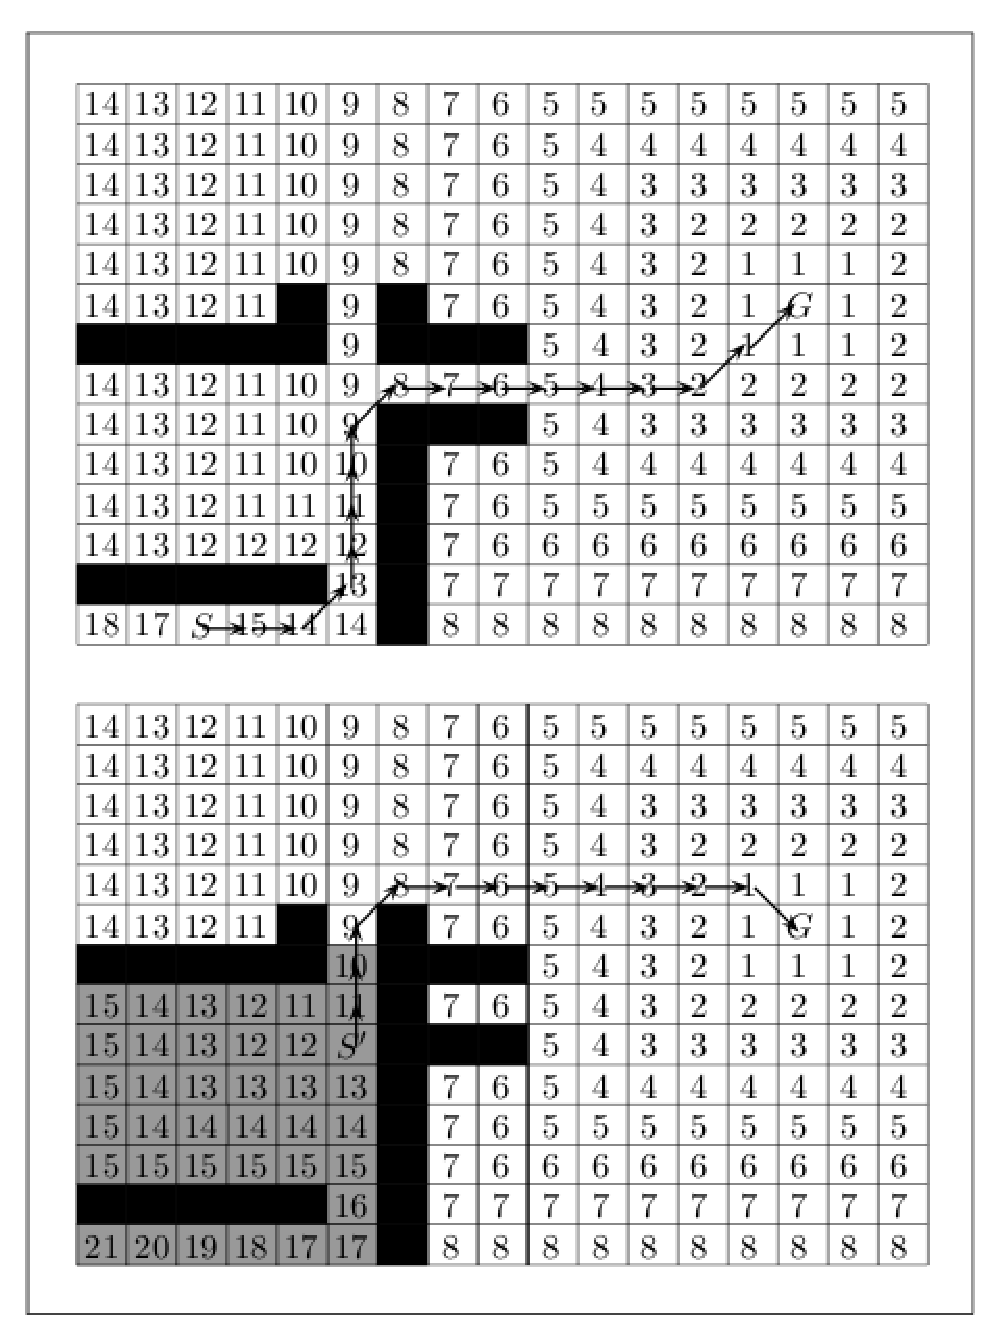
\includegraphics[width=4in]{dstarlite/dStarLiteExample}
\caption{A Simple Grid Search Representation}
\label{fig:dStarLiteExample}
\end{figure}

\subsection{The Algorithm}

This subsection represents the notation, gives details of used core components and elaborates every single step of D* Lite.

\subsubsection{Notation \& Formulation}
The notation is defined for D* Lite as follows: Let $S$ denotes the finite set of vertices of the graph. Let $Succ(s) \subseteq S$ and $Pred(s) \subseteq S$ denote the set of successors and predecessors of vertex $s \in S$, respectively. 

The cost of moving from vertex $s$ to $s' \in Succ(s)$ is denoted by $0 < c(s, s') \leq \infty$. D* Lite always gives shortest path found between $s_{start}$ and $s_{goal}$ where $s_{start}, s_{goal} \in S$. $g^*(s)$ is used to define the distance from $s_{start}$ to a vertex $s$. Heuristic function of D* Lite is also similar with classic A*, where $h(s_{goal}, s_{goal}) = 0$ and $h(s, s_{goal}) \leq c(s, s') + h(s', s_{goal})$; triangular inequality is held for all vertices $s \in S$ and $s' \in Succ(s)$ with $s \neq s_{goal}$.

D* Lite maintains an estimate $g(s)$ of the start distance $g^*(s)$ of each vertex $s$, analogous to the \textit{g-values} of an A* search. D* Lite carries them forward from search to search. D* Lite also maintains a second kind of estimate of the start distances; the \textit{rhs-values} are one step lookahead values based on the \textit{g-values} and thus potentially better informed than the \textit{g-values}. The \textit{rhs-values} should always satisfy the following equation;

\[ rhs(s) = \left\{ \begin{array}{cc}
0 & \mbox{if $s=s_{start}$};\\
min_{s' \in Pred(s)}(g(s') + c(s', s)) & \mbox{otherwise}.\end{array} \right. \] 

A vertex is stated as locally consistent if and only if its \textit{g-value} is equal to its \textit{rhs-value}, otherwise it is locally inconsistent. In the case that all vertices are locally consistent, the \textit{g-values} of all vertices are equal to their start distances, $g^*(s)$ namely. Actually, D* Lite does not try to make all vertices locally consistent after some edge costs have changed. It is not required to recompute start distances which have been computed before and have not been changed. Also, it uses admissible heuristic information in order to focus the planning phase and updates only the related \textit{g-values} which are relevant to the computation of a shortest path.

The D* Lite algorithm is complete; it always finds a shortest path if one exists or terminates. If $g(s_{goal}) = \infty$ after the search, then no path is constructed between $s_{start}$ and $s_{goal}$. Otherwise, one can trace a shortest path from $s_{start}$ to any vertex $s_{u}$ by, starting at vertex $s_{u}$, and always tracing back from the current vertex $s$ to any predecessor $s'$ of $s$ that minimizes $g(s') + c(s', s)$ until $s_{start}$ is reached. Notice that ties are broken arbitrarily.

\subsubsection{Core Components and Details}

Consistency of a vertex in the search graph could be considered in several conditions. A vertex $s$ is called \textit{locally consistent} iff $g(s) = rhs(s)$ and \textit{locally inconsistent} iff $g(s) \neq rhs(s)$. Local inconsistency refers to those whose \textit{g-values} need to be updated to become locally consistent. In the same manner, a locally inconsistent vertex is called \textit{locally overconsistent} iff $g(s) > rhs(s)$ and \textit{locally underconsistent} iff $g(s) < rhs(s)$. These consistency situations are used to manage vertices.

Like A*, D* Lite also maintains a priority queue with heuristic information such that the most promising vertices are expanded first. This queue contains only the locally inconsistent vertices which are selected sequentially to be expanded according to their key values $k(s)$, a vector of two components:
\begin{gather*}
k(s) = [k_{1}(s); k_{2}(s)] \\
k_{1}(s) = min(g(s), rhs(s) + h(s, s_{goal})) \\
k_{2}(s) = min(g(s), rhs(s))
\end{gather*}
The first component of the key $k_{1}(s)$ corresponds to $f(s) = g*(s) + h(s, s_{goal})$ which is the \textit{f-value} of A*, and the second component $k_{2}(s)$ corresponds to the \textit{g-value} of A*. Keys are compared (and maintained in the priority queue) in lexicographic order where $k(s) \leq k(s')$ iff either $k_{1}(s) < k_{1}(s')$ or $k_{1}(s) = k_{1}(s')$ and $k_{2}(s) \leq k_{2}(s')$.

Thus, the key with the smallest value is taken from the priority queue and expanded. The queue has several functionalities; where \textit{top()} returns the vertex with the smallest priority, \textit{topKey()} returns the key value of the vertex at the top or $[\infty, \infty]$ if the queue is empty. \textit{pop()} removes and returns the vertex with the smallest key and finally, the member functions \textit{remove()} and \textit{insert()} removes a vertex from and inserts a vertex into the queue, respectively.

\begin{algorithm}
	\caption{D* Lite Outline}
	\label{algDLite-1}
	%\begin{spacing}{0.5}
	{\fontsize{9}{9}\selectfont
    \begin{algorithmic}[1] % line numbering every line
      \Function{calculateKey}{s}
      	\State \Return $[min(g(s), rhs(s)) + h(s_{start},s) + k_{m} ; min(g(s), rhs(s))];$
      \EndFunction
   	  \Statex
      \Function{initialize()}{}
      	\State $U = \varnothing;$
      	\State $k_{m} = 0;$
      	\ForAll{$s \in S$}
     		\State $rhs(s) = g(s) = \infty;$
     	\EndFor
      	\State $rhs(s_{goal}) = 0;$
      	\State $U.insert(s_{goal}, calculateKey(s_{goal}));$
	  \EndFunction
	  \Statex
	  \Function{updateVertex}{u}
   	  	\If{$u \neq s_{goal}$}
   	  		\State $rhs(u) = min_{s' \in succ(u)}(c(u,s') + g(s'));$
   	  	\EndIf
   	  	\If{$u \in U$} U.remove(u); \EndIf
   	  	\If{$g(u) \neq rhs(u)$}
   	  		\State U.insert(u, calculateKey(u));
   	  	\EndIf
   	  \EndFunction
	  \Statex	  
  	  \Function{computeShortestPath()}{}
      	\While{$U.topKey() < calculateKey(s_{start})$ $||$ $rhs(s_{start}) \neq g(s_{start})$}
      		\State $k_{old} = U.topKey();$
      		\State $u = U.pop();$
    	  	\If{$k_{old} < calculateKey(u)$}
   		  		\State U.insert(u, calculateKey(u));
   		  	\ElsIf{$g(u) > rhs(u)$}
    	      	\State $g(u) = rhs(u);$
				\ForAll{$s \in pred(u)$} updateVertex(s) \EndFor
			\Else
				\State $g(u) = \infty;$
				\ForAll{$s \in pred(u) \cup u$} updateVertex(s); \EndFor
	   	  	\EndIf
      	\EndWhile  	  
  	  \EndFunction
    \end{algorithmic}}
    %\end{spacing}
\end{algorithm}

\begin{algorithm}
	\caption{Cont'd of D* Lite Outline}
	\label{algDLite-2}
	%\begin{spacing}{0.5}
	{\fontsize{9}{9}\selectfont
    \begin{algorithmic}[1] % line numbering every line
	  \Function{plan()}{}
	  	\State $s_{last} = s_{start}$
      	\State initialize();
      	\State computeShortestPath();
      	\While{$s_{start} \neq s_{goal}$}
			\If{$g(s_{start}) = \infty$} there is no known path \EndIf
			\State $s_{start} = argmin_{s' \in succ(s_{start})}(c(s_{start},s') + g(s'));$
			\State Move to $s_{start}$;
   	      	\State Scan the graph for changed edge costs;
    	      	\If{Any weight cost changed}
    	      		\State $k_{m} = k_{m} + h(s_{last}, s_{start}));$
      			  	\State $s_{last} = s_{start};$
    	      		\ForAll {directed edges (u,v) with changed edge costs}
    	      			\State Update the edge cost c(u,v);
    	      			\State updateVertex(u);
    	      		\EndFor
		      		\State computeShortestPath();
    	      	\EndIf
		\EndWhile
  	  \EndFunction
    \end{algorithmic}}
    %\end{spacing}
\end{algorithm}

The D* Lite algorithm is started by calling \textit{plan()} method in Algorithm \ref{algDLite-2}. It first calls \textit{initialize()} in Algorithm \ref{algDLite-1} at $\lbrace 3 \rbrace$ to start the search. \textit{initialize()} sets priority queue \textit{U} to an empty set, the heap reordering variable $k_{m}$ to zero, and the \textit{g} and \textit{rhs-values} of all vertices to infinity. Initially, $s_{start}$ is the only consistent vertex and is inserted into the empty priority queue with its calculated key $k(s_{start})$. \textit{calculateKey()} method is used to calculate the key of corresponding given vertex. Key formulation and generation is indicated above. This initialization guarantees that the first call to \textit{computeShortestPath()} at line $\lbrace 4 \rbrace$ in Algorithm \ref{algDLite-2} performs an A* search that it expands the same vertices as A* would, in exactly the same order.

After first execution of \textit{computeShortestPath()}, a loop is processed until reaching to $s_{goal}$. In each iteration, when $g(s_{goal})$ is observed as $\infty$, one can infer that there is no known path between $s_{start}$ and $s_{goal}$. If this is the case, the algorithm can be terminated. Else, next vertex to move is determined as new $s_{start}$ with the equation in line $\lbrace 7 \rbrace$ in Algorithm \ref{algDLite-2} where minimum cost adjacent of current $s_{start}$.

At this point, a change in the edge costs is waited in the environment at line $\lbrace 9 \rbrace$. If any edge costs have changed, the heap variable $k_{m}$ is cumulatively updated with heuristic function of last visited and $s_{start}$ vertices. Then; for all changed edge costs, new cost $c(s, s')$ is recalculated and \textit{updateVertex()} is called to recompute the \textit{rhs-values} and keys of the vertices potentially affected by the changed edge costs. In addition, if any of the vertices potentially affected have become locally consistent or inconsistent, their membership in the priority queue is adjusted. The $k_{m}$ variable is important because repeated reordering of priority queue $U$ is expensive since it often contains large number of vertices. By cumulatively adding heuristic value between last visited vertex and start, whenever new priorities are computed, the variable $k_{m}$ has to be added to key value's first components. In this way, the order of vertices in the priority queue is unaffected when the agent moves and the priority queue doesn't need to be reordered.

Finally, \textit{computeShortestPath()} is called which repeatedly expands locally inconsistent vertices according to their priorities. If top key of $U$, $k_{old}$ is smaller than calculated new key of corresponding vertex $u$, this vertex is inserted into queue. When it expands a locally overconsistent vertex $u$ at $\lbrace 22 \rbrace$ in Algorithm \ref{algDLite-1}, \textit{g-value} is set as \textit{rhs-value} to make $u$ locally consistent. When a locally underconsistent vertex $u$ is expanded in $\lbrace 25 \rbrace$, the \textit{g-value} of $u$ is set to infinity. This makes the corresponding vertex $u$ either locally consistent or overconsistent. If it was locally overconsistent, then changing of its \textit{g-value} can effect the local consistency of its neighbours, or successors. Otherwise, if $u$ was locally underconsistent, then changing of its \textit{g-value} can effect the local consistency of itself and its neighbours. As a result, \textit{computeShortestPath()} must \textit{updateVertex()} for all of the vertices potentially effected by the change in their \textit{g-values}. It modifies their \textit{rhs-values}, checking their consistency, and adding them to or removing them from the priority queue as appropriate in \textit{updateVertex()} method in lines $\lbrace 10 - 15 \rbrace$. The vertices are expanded by \textit{computeShortestPath()} until the key of the next vertex $s'$ to be expanded is no less than that of $s_{goal}$ or until $s_{goal}$ is locally consistent. This behaviour is similar with A* where expands vertices until it expands $s_{goal}$ at which point the \textit{g-value} of $s_{goal}$ is equal to its start distance and the \textit{f-value} of the node to expand next is no less than the \textit{f-value} of $s_{goal}$.

At the end of the algorithm execution, one can trace back a shortest path from $s_{start}$ to $s_{goal}$ by always transitioning from the current vertex $s$, starting at $s_{goal}$ , to any predecessor $s'$ that minimizes $g(s') + c(s',s)$, breaking ties arbitrarily, until $s_{start}$ is reached.
\newpage

\chapter{Partially Observable Markov Decision Processes and Factored Representations}
\label{chapter:background}

In this chapter, we presented the fundementatl concepts on Partially Observable Markov Decision Processes and factored represenation schemas used to represent and efficiently solve POMDP problems.

\section{Markov Decision Processes}

Markov Decision Process (MDP) is a framework for studying decision making problems in probabilistic domains.

An MDP is based on stochastic processes, decision problems and Markovian property.

Probabilistic decision making can be modeled similar to a stochastic process. In AI perspective an agent interacts with an environment and after each action executed by the agent, environment changes in a probabilistic way.

The Markovian property indicates that, at any state, the following state will not be related to previous states. Formally,

\begin{displaymath}
\Pr(s^{k+1} | s^{k}, s^{k-1}, \ldots , s^0) = \Pr(s^{k+1} | s^{k}). \,
\end{displaymath}

A decision problem with a Markovian property has distinct states and at each state the following states are determined by actions taken and world dynamics. Most of the probabilistic decision problems fall into this category. In general for real-life problems and even for simple demonstrative problems, different histories of execution that lead to the same state have no distinct importance.

Also, the Markovian property reduces the solution complexity, since a solution attempt does not have to deal with execution histories.

\subsection{Formulation}

An MDP is formulated as

\begin{itemize}
\item Set of state space, $S$
\item Set of actions, $A$
\item State transition function, $T : S \times S \times A \to [0,1]$
\end{itemize}

These three factors determine \emph{how the world changes}. As the nature of a decision problem dictates, some states are desirable and some states are not desirable in an MDP. Reward function captures this notion.

\begin{itemize}
\item Reward Function, $R : S \times S \times A \to \mathbb{R}$
\end{itemize}

$T(s, s', a)$ is the probability that taking action $a$ at state $s$ leads to state $s'$. $R(s, s', a)$ is the amount of reward received \emph{immediately} when system changes from state $s$ to state $s'$ via action $a$.

\subsection{Deterministic Case}

When state transition function is formulated as

\begin{displaymath}
T : S \times A \to S
\end{displaymath}

or

\begin{displaymath}
T : S \times S \times A \to \{0,1\}
\end{displaymath}

the system is deterministic, i.e. there is a single next state for a given state-action pair. In this setting the problem reduces to a classical planning problem.

\subsection{Acting on an MDP Problem}

In AI perspective, an agent acting on an MDP reacts to the environment via $S, A, T$ and $R$. At any state $s$, agent chooses an action among $A$. This action changes the world, according to $T$ and the world enters a new state $s'$. Agent is noticed the reward received upon this transition. Thus, a time-tick is completed. Agent now chooses a new action for $s'$.

An execution history is a string of states and actions of such an agent acting on an MDP. It is a snapshot of lifetime of an agent in a given time frame.

\begin{displaymath}
H = s^0a^0s^1a^1s^2 \ldots a^{n-1}s^{n}
\end{displaymath}

The cumulative reward gained at such an execution history is the sum of rewards gained at each step.

\begin{displaymath}
Cumulative Reward(H) = \sum_{i=1}^{i=n} R(s^{i-1}, s^i, a^{i-1})
\end{displaymath}

The agent may decide which action to take according to its internal architecture. For MDP problems, it is assumed that the agent knows all problem dynamics ($S, A, T$ and $R$) perfectly. Also it is assumed that at each time-tick, the new state $s'$ is perfectly observable by the agent (See Section \ref{section:pomdp} for generalization). For MDP problems general practice is constructing a policy in form of a mapping from states to actions. Thus acting on an MDP environment is simply executing the action that the policy dictates for the current state.

\subsection{Solving an MDP Problem}

In simple terms, solving an MDP problem is finding a way to act optimally.

The optimality is measured generally in terms of cumulative reward. Cumulative reward of an execution history might be quite precise to measure the optimality of a solution. However there are two factors that complicate this view:

\begin{enumerate}
\item There is an infinite number of execution histories, since there is no boundary for the length of an execution history and the formulation of MDP does not specify any concept of termination.
\item Even considering execution histories of some fixed length, since state transition is probabilistic in nature, applying same actions starting with the same initial state might lead to different execution histories.
\end{enumerate}

Since there are infinitely many execution histories, it is essential to formulate an \emph{expected cumulative reward} of a policy $\delta$, given a fixed execution history length $t$ (which is commonly called \emph{horizon}).

\begin{displaymath}
\begin{array}{rl}V_t^\delta (s) = \sum_{s'} T(s ,s', \delta(s)) [ R(s, s', \delta(s)) + V_{t-1}^\delta (s')]  & t>0 \\
& \\
V_0^\delta (s) = \sum_{s'} T(s, s', \delta(s)) [ R(s, s', \delta(s)) ]\end{array}
\end{displaymath}

$V_t^\delta (s)$ is the expected cumulative reward of applying policy $\delta$ for $t+1$ steps, starting at state $s$.

\subsection{Algorithms for Solving MDP Problems}

\subsubsection{Value Iteration}

\emph{Value Iteration} is a dynamical programming method used in learning and decision problems. The pseudocode for the algorithm is given in Figure \ref{figure:valueiterationalgorithm}.

In a state oriented view of the world each state has a value, based on the reward received at that state, and possible next states. Value Iteration algorithm tries to approximate this value iteratively. Modified version of value iteration algorithms try to approximate value of state-action pairs.

In a dynamical system, value of a state is the expected cumulative reward gained after that state. It is possible to formulate this statement recursively. At a given state, there are finite number of possible next states, even we do not have a restriction for the action taken. Thus, if we know the value of all the next states, we can calculate the value of the current state.

Below formulation is used for calculating expected cumulative reward with an arbitrary horizon $t$:

\begin{displaymath}
\ V_t^\delta (s) = \sum_{s'} T(s ,s', \delta(s)) [ R(s, s', \delta(s)) + V_{t-1}^\delta (s')]
\end{displaymath}

We can use this formula for finding the real value function, $V^*$.

Then we find the $V^*$, $\delta(s)$ follows as:

\begin{displaymath}
\ \delta(s) = \underset{a}{\mbox{argmax}} \sum_{s'} T(s,s',a) [ R(s, s', a) + V^* (s')]
\end{displaymath}

With combining these two ideas, we can formulate an algorithm to calculate $V^*$. Algoritm starts with an initial random guess of $V^*$, called $V^0$ \footnote{It's important not to confuse this superscript with the numerical subscript used to indicate the horizon of the function.}.A refined version of $V^0$, $V^1$ can be constructed by using the cummulative reward formula and using $V^0$ for value of the next state (operator $:=$ symbolizes ''update'')

\begin{displaymath}
\ V^1(s) := \sum_{s'} T(s ,s', \delta(s)) [ R(s, s', \delta(s)) + V^0 (s')]
\end{displaymath}

It's usually preffered to use a discount factor $\gamma (0 < \gamma < 1)$ to speed up the convergence to $V^*$:

\begin{displaymath}
\ V^1(s) := \sum_{s'} T(s ,s', \delta(s)) [ R(s, s', \delta(s)) + \gamma . V^0 (s')]
\end{displaymath}

Thus the actual reward values influence $V^1$ more then $V^0$ values.

Since delta formula and this formula are similar, it is possible to rewrite this formula with eliminating delta:

\begin{displaymath}
\ V^1(s) := \max_a \sum_{s'} T(s ,s', a) [ R(s, s', a) + \gamma . V^0 (s')] \qquad (0 < \gamma <1 )
\end{displaymath}

Note that this formula should be applied to each state. At each application, we have a maximization over all actions and we have a summation over all states. Generalizing this formula we have:

\begin{displaymath}
\ V^{k+1}(s) := \max_a \sum_{s'} T(s ,s', a) [ R(s, s', a) + \gamma . V^k (s')] \qquad (0 < \gamma <1 )
\end{displaymath}

We can apply this formula repeatedly to find better approximations to $V^*$. It is possible to show that this iteration converges to $V^*$, if it exists.

It's also possible to forget to maintain separate $V^k$ and $V^{k+1}$ values, or we can use a dynamic programming approach, eliminating the indexes and iterating continously for all states:

\begin{displaymath}
\ V(s) := \max_a \sum_{s'} T(s ,s', a) [ R(s, s', a) + \gamma . V (s')] \qquad (0 < \gamma <1 )
\end{displaymath}

When $V$ converges to $V^*$, right and left sides of the formula get equal and no update is done. Thus, it is possible to terminate the iteration by examining the '''update amount''':

\begin{displaymath}
\ \Delta := \max_s | V(s) - \max_a \sum_{s'} T(s ,s', a) [ R(s, s', a) + \gamma . V(s')]
\end{displaymath}

When $\Delta$ gets low enough, algorithm is terminated.

\begin{algorithm}
\SetLine
   Initialize $V$ arbitrarily, e.x. $V(s) := 0$, for all s\;
   \Repeat{ $\Delta < /Theta$ }{
	   $\Delta := 0$\;
	   \ForEach {$s \in S$} {
		   $\ v := V(s)$\;
		   $\ V(s) := \ \max_a \sum_{s'} T(s,s',a) [R(s,s',a) + \gamma . V(s')]$\;
		   $\ \Delta := \max (\delta, | v - V(s) |)$\;
	   }
   }
   $\ \delta(s) = \underset{a}{\mbox{argmax}} \sum_{s'} T(s,s',a) [ R(s, s', a) + V^* (s')]$\;
\caption{Value Iteration Algorithm}\label{figure:valueiterationalgorithm}
\end{algorithm}

Each iteration of Value Iteration Algorithm (Do-While loop) takes $\ \mathcal{O} (|S|^2|A|)$ operations, due to maximization on actions and summation over next state. The number of iterations is polynomial in terms of $|S|$.

\subsection{Q-Learning Algorithm}

It's sometimes preferable to refine the value function and define it from $S \times A$. So instead of $V(s)$ we have $Q(s,a)$. A similar iterative algorithm can update Q values.

\begin{displaymath}
\ Q(s,a) := \sum_{s'} T(s ,s', a) [ R(s, s', a) + \gamma . V (s')] \qquad (0 < \gamma <1 )
\end{displaymath}

At each iteration of the formula, we should apply it to all ''state-action pairs''.

The advantage of Q-Learning Algorithm is, we know the exact value of each action at each state.

Q-Learning algorithm has the same time complexity with the Simple Value Iteration Algorithm. However if we are using dynamic programming, the size of the Q-table is $\mathcal{O} (|S||A|)$ which is much bigger then an ordinary value table. And more importantly the extra information that the Q values supply is redundant for solving an MDP problem. It is possible to deduce a policy without this extra knowledge.

Q-values becomes important if the problem is a learning problem, where state transition function is unknown to agent (as the name Q-Learning suggests). For such problems, it is not possible to maximize over all actions, unless the agent has not executed them and perceived the actual next state. So it is not easy to apply Value Iteration algorithm. Since Q-Learning does not have a maximization over actions, traces of agent's actions can be fed into Q-update rule as $(s,s',a)$ triplets.

\subsection{Policy Iteration}

\emph{Policy Iteration} is an algorithm based on improving a policy for a learning problem or a decision problem.

The main idea behind policy iteration is, given a policy, it is possible to calculate a value function based on this policy. And given a value function, it is possible to refine the policy.

Policy Iteration Algorithm is similar to Value Iteration, in the sense that both algorithms try to improve the solution in iterations. Solution of Policy Iteration Algorithm is policy itself.

Policy Iteration Algorithm starts with an initial arbitrary policy $\pi$. Each iteration of algorithm has two phases:

\begin{enumerate}
\item Value Calculation Phase
\item Policy Improvement Phase:
\end{enumerate}

\subsubsection{Value Calculation Phase}

In this phase the value function of the policy $\pi$ is calculated. The classical value function formula is sufficient for this calculation:

\begin{displaymath}
\ V_\pi(s) = \sum_{s'} T(s, s', \pi(s)) [ R(s, s', \pi(s)) + \gamma . V_\pi(s') ]
\end{displaymath}

Writing this equation for each $s \in S$ gives us $|S|$ different equations. $V_\pi(s)$ and $V_\pi(s')$ are unknowns in these equation, for each $s,s' \in S$. We have a linear system of $|S|$ variables and $|S|$ unknowns, it is possible to find a solution. The solution for $V_\pi(s)$ gives us value function of the policy.

\subsubsection{Policy Improvement Phase}

It is possible to create a refined version of the policy by using the value function. This phase is identical to policy extraction step of Value Iteration algorithm.

\begin{displaymath}
\ \pi'(s) := \underset{a}{\mbox{argmax}} (\sum_{s'} T(s,s',a) [ R(s,s',a) + \gamma . V(s')])
\end{displaymath}

\subsubsection{Termination Condition}

When policy converges to optimal policy, value function calculated at the first phase converges to optimal value function. Thus the refined policy extracted at the second phase is the optimal policy again.

This fact gives us a sufficient termination condition. When an iteration does not refine the policy anymore, i.e. refined policy is equal to the original one, the algorithm terminates, converging to optimal policy.

\subsubsection{Computational Complexity of the Algorithm}

Each iteration of the Algorithm has two phases. Value Calculation phase is simply solving a linear system with $|S|$ equations. This phase has polynomial complexity, specifically $\mathcal{O}(|S|^3)$ if Gaussian Elimination is used. Policy Improvement phase has complexity $\mathcal{O}(|S|)$.

At the worst case, the policy algorithm iterates over all possible policies until finding the optimal one. Since there is $|A|^{|S|}$ possible policies, the number of policies have exponential complexity. However it is shown that the running time is pseudo polynomial\cite{littman95}.

\section{Partially Observable Markov Decision Processes}
\label{section:pomdp}
A POMDP is a framework for modeling probabilistic decision making problems featuring partial observability.
The framework is similar to MDPs, where there is no partial observability and the state information is known
perfectly. However, in the POMDP framework, it is not possible to observe the state perfectly, instead an
imperfect observation~is~available \cite{Kaelbling98,Cassandra94,Cassandra98}.

The model is formulated as

\begin{itemize}
\item Set of state space, $S$
\item Set of actions, $A$
\item State transition function, $T : S \times S \times A \to [0,1]$
\end{itemize}

These model elements are identical to elements of an MDP. The distinction between MDPs and POMDPs is in a POMDP system any executing action does not have any knowledge about current world state $s \in S$. An agent acting on a POMDP perceives an ''observation'' at each time-tick, which is different than the state information.

\begin{itemize}
\item Set of observations, $O$
\item Observation function, $\O : S \times A \times O \to [0,1]$
\end{itemize}

The observation function is a function of observations, states and actions, gives the probability of perceiving given observation ''after'' the world goes to given state with the effect of given action. The reward function is also a function of observations, reward given at any time-tick is dependent to the observation perceived.

\begin{itemize}
\item Reward Function, $R : S \times S \times A \times O \to \mathbb{R}$
\end{itemize}

The major impact of partially observability is that the system no longer has the Markovian property ''by agent's view''. The underlying state based model is still Markovian. However observation based view of the system does not hold this property. Any observation to be perceived in the future is not only dependent to current observation, since this current observation might not uniquely map to the current state. Different observation might be perceived at any state and an observation might be perceived at a number of states.

Also since the observations are probabilistic it is not generally possible to establish a mapping between states and observations. Still some of the solution methods try to establish such a mapping, even if it is probabilistic.

An agent acting on a POMDP problem has a similar view with the MDP version. The only major difference is the agent perceives an observation at each time-tick, instead of a new world state. Thus an execution history has form

\begin{displaymath}
H = o^0a^0o^1a^1o^2 \ldots a^{n-1}o^n
\end{displaymath}

at agent's perspective.

Since the reward function is dependent to state information and state information is inaccessible to agent, it is not possible to calculate a cumulative reward in any way except summing the actual rewards. Thus reward information might be added to execution history.

\begin{displaymath}
H = o^0a^0r^0o^1a^1r^1o^2 \ldots a^{n-1}r^{n-1}o^n
\end{displaymath}

Solving a POMDP problem is still about finding a way to act optimally. For POMDP problems, an agent may act upon a policy but it is not possible to construct a policy simply as a mapping.

It is possible, however worthless, to construct the policy as a state-action mapping since state information is not accessible. Then the policy should also contain a way to determine the current state to use this state-action pair.

It is not possible to construct the policy as an observation-action mapping since this view does not hold the Markovian property and current observation does not implicate current state.

Since these approaches should not work, it is necessary to construct a more sophisticated policy for agents acting at POMDP problems.

Since there is no simple policy structure for a POMDP, it is also not possible for a simple optimality metric. The principal of optimality is same with the MDP case. A policy is optimal if and only if expected cumulative reward received by applying the policy is optimal. Calculation of expected cumulative reward should be similar to MDP case for any policy type. It is important to note that next state should be dependent to observations too.

\subsection{Algorithms for Solving POMDP problems}

\subsubsection{History Based Algorithms}

Most important challenge of solving POMDP problems is their lack of Markov property, in terms of observations and actions. However, if an execution history is available, it can be used for defining a new MDP problem in terms of history states.

In order to apply a history based algorithm, one should have sufficient history data on all the state space. Thus an history-based algorithm can be configured in a generative way, which involves producing history data from known world dynamics; or it can be configured as a learning problem.

Set of states of the new problem is strings of execution histories of the POMDP problem, containing alternating actions and observations.

Set of actions of the new problem is set of action of the POMDP problem.

An important probability function is ''belief state probability function'', which is a probability distribution of current state, given a history-state. This function can be computed iteratively, by using initial state distribution, state transition function of POMDP and observation distribution function of POMDP.

Transition function of the new problem is defined as probability of perceiving an observation of POMDP problem, given a history-state and an action. New state is just the history-state, concatanated with given action and observation. This transition function can be computed using transition and observation functions of POMDP with ''belief state probability function''.

Reward function of the new problem is similarly probability of receiving a certain reward after executing a given action at a given history-state. This function can be computed using original reward function and observation distribution functions of POMDP with the ''belief state probability function''

The calculation of both functions just consists of taking expected value over the ''belief state probability function''.

With all the components of an MDP system, the new derived MDP problem can be solved using Value Iteration or any other MDP solving method.

This approach is successful in the sense that, even we don't know the transition and observation distributions of the POMDP, we can generate estimates from the execution history and use them in the algorithm. This algorithm can be constructed as a pure model-free method to solve a POMDP online.

However it is apparent that the state space of the constructed MDP is exponential in terms of state and action spaces of the original POMDP.

\subsubsection{Belief State Based Algorithms}

History-state based approach has a huge state space and a simpler approach is possible if the system dynamics are well known. When the transition function and and observation function are known, ''belief state probability function'' can be used to maintain a policy.

The general approach of all belief state based algorithms is similar to the Value Iteration algorithm of MDP problems. As state information, we have belief states, which is the domain of the ''belief state probability function''. A belief state can be formulated as a vector.

The value function over belief states is a piecewise linear function. So similarly value function can be represented as a set of $n$ dimension vectors, too.

With such vectorial representation, value of an arbitrary belief state, w.r.t to value function is the maximum value of the dot product of each vector in value function with the belief state vector.

It is possible to use Value Iteration and find the vectors that form value function. However there is one important obstacle, the belief state space is the set of all $n-dimensional$ probability distribution vectors, and this state space is a continuous one. It is known that the problem is inherently a discrete problem, however discritizing the continuous belief state space is a difficult problem.

Different algorithms are proposed for maintaining a discrete view by using the Value Iteration.

\begin{itemize}
\item Sondik/Monahan's Enumeration Algorithm tries to enumerate all possible useful belief states and apply Value Iteration algorithm only considering these belief states.
\item Sondik's One Pass Algorithm tries to find a value function component for a single belief state, and then explore the belief state interval, on which this component of value function is dominating by examining possible actions and outcomes.
\item Cheng's Linear Support Algorithm tries to build the Value Function directly.  The approach is similar to the One Pass Algorithm, however Linear Support Algorithm relies of geometric properties of Piecewise Linear Value Function, rather then using possible actions and their outcomes.
\item Witness Algorithm is similar to Linear Support Algorithm, but it also uses observations in order to simplify the calculation of real value of belief points.
\end{itemize}

\section{Factoring of POMDP Problems}

\subsection{Factored MDP and POMDP}
There are a number of challenges, of which all POMDP algorithms, especially belief based ones, suffer from:

\begin{itemize}
\item Continuity of belief space is an important challenge for belief based POMDP algorithms. A belief based algorithm has to find a way to deal with the continuous space as a first task. Luckily a value function of a PODMP problem is a piecewise linear and we have a simple finite mean to represent it. This also allows overcoming the challenge of the continuity.
\item \emph{Curse of Dimensionality} is the difficulty of manipulating value function for huge problems, which have many states and actions. Value function should be calculated by considering all states and actions even in the simples possible form. Thus huge number of states and actions increases both the size of value function and time/space necessary to compute it.
\item \emph{Curse of Horizon} is an effect of Curse of Dimensionality. Most of the problems proposed for POMDP problems are iterative. Each iteration produces a policy for a specific horizon. At each iteration, horizon is increased. Since the horizon increases, each iteration deals with a more complex belief state, a more complex value function. We can simply say that Curse of Dimensionality gets worse as the horizon increases.
\end{itemize}

It is possible to formulate more efficient algorithms to overcome this issues. However one of the underlying reasons of these difficulties is POMDP models use representations more inefficient then should be. Most of the real life problems do not have distinct unique states, actions and observations. Most of the real world problems exhibit some structure in action space, state space and observation space \cite{schut02}.

Factored POMDPs could be seen as the most important attempt made to exhibit the structure of POMDP
problems~\cite{Boutilier95}. The idea was originally used for MDP problems. Instead of representing the
problem with a set of states and actions, the factored approach represents MDP problems with ``state
variables'' and actions. The state notion is simply the cross product of all state variables. This idea is
also applicable to POMDP problems where the state space is only partially observable. Partial observability
provides a natural factorization among states. This is known as mixed observability. Using factorization
structure of the state space can be used to simplify the problem~\cite{Smith07, Kveton06}. Our intention is
to use the factored PODMP in tackling the GRN control problem. 

Factored POMDP can be demostrated by using an example problem. For this purpose we used RockSample problem. RockSample is a simple 2-D robot problem. A robot is navigating in an obstacle free environment with some rocks available to collect. Some rocks have value and others do not. The robot knows its location and the locations of rocks, but does not know the quality of rocks, which makes the problem partially observable. The robot can use its long range sensor to determine the value of any rock. The sensor reading is noisy proportional to the distance to the rock sensed. The robot have specific start and goal locations.

In our examples a 4x4 environment RockSample problem is used with 4 rocks in the environment.

For RockSample domain, a possible representation is

\begin{itemize}
\item $S = \{ L , RQ1, RQ2, RQ3, RQ4\}$ where $Val(L) \in \{(a,b) | 1 \le a,b \le 4\}$ and $Val(RQ1),Val(RQ2),Val(RQ3),Val(RQ4) \in \{havevalue, novalue\}$
\item $A = \{ ML, MR, MU, MD, SR1, SR2, SR3, SR4, G\}$
\item $O = {SR}$ where $SR \in {positive, negative}$
\end{itemize}

In this representation, $L, RQ1, RQ2, RQ3$ and $RQ4$ are state variables where $L$ is the location of agent, $RQ1,RQ2,RQ3$ and $RQ4$ are qualities of 4 rocks in the environment. Action set contains four actions for moving ($M MR, MU$ and $MD$), four actions for sensing the rocks in the environment ($SR1, SR2, SR3$ and $SR4$) and a grab action to collect the rock at the agent's location. After trying to sense any rock in the environment, agent receives an observation of positive or negative. Without activating the senses, agent does not receive any observation.

The transition function is deterministic and the observation function has probabilities associated with sense actions dependent to the distance between the agent and the sensed rock.

The reward function maps +10 reward to sampling a rock with value, -10 reward to sampling a rock without value. Also the reward function maps +10 to reaching the goal location.

This representation is previously used for algorithms working on Factored representation of POMDP problems. There is only single modification we made . We did not used extra observations or extra rewards for reinforcing the agent not to execute illegal actions. Generally to provide homogeneity in problem description, such minor modifications are embedded as extra observations or extra rewards. However our aim is not homogeneity, on the contrary, to partition the problem using the structure it exhibits. So we were fine with omitting such modifications for the sake of homogeneity.

Last element of the factored representation is determining the relations between state variables in the given problem description. It is possible to use Dynamic Bayesian Networks for this purpose.

Figure \ref{figure:rocksample} depicts the factored representation of RockSample problem. Each part of the figure presents the world and observation dynamics for a single action. For any action that involves moving (in particular $ML$ for the figure), only the state variable $L$ changes. For any action that involves sensing rock quality (in particular $SR2$ for the figure) the value of the onservation perceived is determined by the actual quality of the rock and the location of the agent. No state variable changes for this action. Finally grab action possibly changes all the rock quality state variables, depending to the location of the agent. If the agent is adjacent to a certain rock, after grabbing the rock quality variable related to that rock will change while other variables remain the same; if the agent is not adjacent to any rock, no rock quality variable will change.

\begin{figure}
\begin{displaymath}
\entrymodifiers={++[o][F-]}
\fbox{\xymatrix{
*\txt{ML} \\
L_{t-1} \ar[r] & L_t \\
RQ1_{t-1} & RQ1_t \\
RQ2_{t-1} & RQ2_t \\
RQ3_{t-1} & RQ3_t \\
RQ4_{t-1} & RQ4_t
}}
\qquad
\fbox{\xymatrix{
*\txt{SR2} \\
L_{t-1} \ar@/_20pt/[ddddd] & L_t \\
RQ1_{t-1} & RQ1_t \\
RQ2_{t-1} \ar@/_20pt/[ddd]& RQ2_t \\
RQ3_{t-1} & RQ3_t \\
RQ4_{t-1} & RQ4_t
\\
SR
}}
\qquad
\fbox{\xymatrix{
*\txt{G} \\
L_{t-1} \ar[dr] \ar [ddr] \ar[dddr] \ar[ddddr] & L_t \\
RQ1_{t-1} \ar[r] & RQ1_t \\
RQ2_{t-1} \ar[r] & RQ2_t \\
RQ3_{t-1} \ar[r] & RQ3_t \\
RQ4_{t-1} \ar[r] & RQ4_t
}}
\end{displaymath}
\caption{Factored dependencies of the problem}\label{figure:rocksample}
\end{figure}

\newpage

\chapter{POMDP Model Formulation for GRN Control Problem}
\label{chapter:formulation}

In order to use the POMDP model for handling a partially observable GRN control problem in hand, we need to
define each model element in terms of the GRN control problem. Our goal is to solve the formulated POMDP
problem by using a conventional POMDP solver. However, we intend to decompose the problem into subproblems
before attempting to produce a solution; and we intend to make use of the factored representation in this
decomposition. Thus, the POMDP model formulation presented in this paper constructs a factored~POMDP.

\section{States}
A joint expression level vector of all genes in the network is a state in the sense of representing the gene
expression control problem as a POMDP. For a flat representation of states, we need to consider all the joint
expression level space. However, for a factored representation, it is easy to represent each gene as a state
variable.

The most important question about accuracy of this state representation is whether all the necessary genes
are included in this expression level network. In the ideal sense, since we do not know all the interactions
in the cell, we can never be certain that the expression level of a gene that is not included in the problem
does not affect the problem. However in reality, for known problems it might be possible to identify related
genes, and we can assume that the state vector contains all genes related to the control problem. This
assumption might be crude for the gene expression control problem, but the assumption is strong in the
generalized case.

Another important point to consider is related to components of the gene expression vector. The source for
gene expression levels is generally experimental data, possibly from multiple sources. The data format only
affects the solution process. However, if the gene expression levels are continuous then we have a continuous
state POMDP, and this should be taken into consideration. In gene expression, there is not much distinction
between minor differences in the expression of a gene. And for the general case, it is possible to restrict
the ideas here to discrete state POMDP problems. In this work, we assumed all gene expression levels are
discretized to a multi-value set.

In all examples and experiments, we used a binary set for discretizing gene expression levels. So each state
variable has two values: \texttt{off} and \texttt{on}. For a network of $n$ genes, we have $n$ state
variables in factored form, each with $2$ values; this corresponds to $2^n$ states for a flat representation.

\section{Actions}
Actions in the gene expression control problem are intervening with the network, setting expression levels of
some inputs. These inputs might be any biological agent. As long as the input is part of the network and the
relationship between the input and any of the genes can be expressed as the relationship between two genes,
the biological characteristics are not significant.

In this work, we assume that some of the nodes in the GRN can be controlled directly. There are no joint
actions. Each action sets the expression level of a single gene either \texttt{off} or \texttt{on}. We also
assume that action \texttt{noop} is available to represent the case of not intervening with the dynamics of
the network. The set of actions are specified as control parameters.

\section{Transition Function}
The transition function of the gene expression control problem expresses the interaction between genes. The
gene expression problem itself does not dictate a transition function. Given a graph of the gene expression
network, it is possible to formulate a transition function using the graph structure.

However, it is also possible to deduce the transition function by using the gene expression data available. We developed a method for analyzing the gene expression data and extracting state transitions by using the available analysis results. This method has two advantages :
\begin{inparaenum}[\itshape i\upshape)]
\item Since already computed values are used there is no need to re-process the data;
\item using analysis results leads to a formulation more consistent with the decomposition, which is also done using the analysis results.
\end{inparaenum}
 The details of the method are described in Chapter~\ref{chapter:dataanalysis}.

In the ideal case, this transition function forumlation is an approximation and we can never be sure 
that the constructed transition function captures all the relationships between genes. However, this 
is a minor problem for transition functions, since we can use methods that construct a transition function 
that models the premises (the graph of the GRN or the gene expression data) as close as possible. Assuming 
our construction actually builds a closed model, the only reason behind missing influences in the transition 
function could be imprecise premises. We may have the chance for building up better premises to construct 
the transition function.  However, if it is not the case, we have to stick to the premise in hand, 
and we have to model a transition function that fits the premises as much as possible.

\section{Observations and Observation Function}
\label{section:observation}
The gene expression problem has many unknown components in reality. Most of the time, what we know about
genes are one of the following two items:

\begin{itemize}
  \item Gene expression data that describes expression levels of a set of genes as snapshots
  \item Correlations between expression levels of genes, derived from biological research
\end{itemize}

In order to formulate a model for GRNs, it is common practice to use any modeling structure and to assume
that such structure approximates the GRN. If the dynamics of the system is accessible from the point of view of a manipulator, then the problem is
 fully observable. This approach is successful in modeling simple
isolated gene expression networks; it is capable of producing policies for controlling the modeled networks.
If we focus on representing GRNs as MDP problems, this modeling approach assumes that the GRN is fully
observable. The generated policies are expressed in terms of the expression levels of genes. This view is
only sound under certain assumptions. In reality, there are a number of aspects that are not fully
observable; some possible scenarios are described next:

\begin{enumerate}
\item The gene regulatory network modeling the interactions between genes is usually deduced from gene
expression data by computational methods, or empirically. Regardless of the confidence level of the method
used, there is always room for error and the actual interaction scheme between genes can not be fully
observed.

\item The traditional biological approach explains certain processes in the cell by pathways. Each gene causes another gene to get activated or suppressed and at the end of the chain reaction a target gene is activated. The control policies defined on simple linear pathways are simply intervening with the gene that starts the chain reaction.

Since there is no restriction on the interactions between genes, more complex interactions are possible. The
control problem turns to be more complicated in many ways when the interactions between genes become more
complex. When the problem becomes more complicated, one important point related to observability is the fact
that only more complicated policies can achieve optimal or near-optimal results for the control problem.
Typically, a more complicated policy requires monitoring the gene expression levels when executing the
policy, and taking different actions for different situations. This is not a strong assumption. When
intervening with a set of genes; generally it might not be possible to observe the activation levels
simultaneously.
\end{enumerate}

If we concentrate on the second factor mentioned here, instead of defining the control problem as fully
observable, it is more realistic to identify an observation set. This observation set is typically direct or
indirect information on the expression levels of some genes. One might be the capability to monitor the
expression levels of some of the genes directly, or via some marker related to the controlled genes.

Of course, for modeling the problem as POMDP, we also need to build an observation function. The observation
function is directly related to the definition of the observation set. However, there is one important thing
to mention here: each observation on the GRN is related to a single gene if the observation is simply the
expression level of a gene. Then, the observation function can be defined trivially. It might be possible to
define more complex observations (e.g., a marker that is related to two genes and observed only when both
genes are expressed) and thus the observation function might get more complicated.

In this work, we assume that a given proper subset of genes in the GRN are observable and this observation is
perfect. Other genes in the GRN are not observable and we do not have any direct information on their
expression levels. The set of observable genes are specified as control parameters.

\begin{equation}
\O(s,a,o) = 
\begin{cases} 
1 & \text{if } \forall g \in O, s(g) = o(g), \\
0 & else
\end{cases}
\end{equation} 

\section{Reward Function}
Generally, the goal of controlling a gene regulatory network is to satisfy some condition over genes (e.g.,
prevent the expression of a gene, provided that two genes are expressed inclusively). This condition can be
expressed as a boolean expression. If the state representation is discrete, it is possible to enumerate
states satisfying the goal. In general, it is always possible to test a state in order to determine whether
it satisfies the goal.

In this work, we use a reward template which is specified as follows:
\begin{equation*}
R(s,a) =
\begin{cases}
\alpha & \text{if $goal(s)$ and $a = noop$,}\\
\alpha-1 & \text{if $goal(s)$ and $a \ne noop$,}\\
0 & \text{if $\neg goal(s)$ and $a = noop$,}\\
-1 & \text{if $\neg goal(s)$ and $a \ne noop$.}
\end{cases}
\end{equation*}

This reward template is based on two factors: (1)~whether the goal description is satisfied or not, and
(2)~the action executed; the \emph{noop} action is a special \emph{no action}. It is possible to read this
template as a linear combination of two reward templates. The goal reward template assigns reward $\alpha$
whenever the goal description is satisfied and the action reward template assigns reward $-1$ whenever an
action is executed. Since these two events are independent, their summation is used as the general reward
template. If the goal description is satisfied, a reward of $\alpha$ is granted, reduced by 1 whenever an
action is executed. Similarly, no reward is granted when the goal is not realized, even reduced by $-1$
whenever an action is executed.

In the experiments, we typically used $\alpha=10$. The ratio of this value and the cost of an action~(1~in
this work) determine the significance of satisfying the goal compared to the cost of intervention; it is a
parameter of the control problem that should to be specified.


\newpage

\chapter{Gene Expression Data Analysis and Formulation Steps Based on This Analysis}
\label{chapter:dataanalysis}

In this chapter, we present details of the gene expression data analysis method used in our work. The goal of
this method is exploring similarities between state variables, and then use these similarities in formulating
a more compact POMDP that utilizes actual behavior of the system.

\section{Gene Expression Data Analysis}
\label{section:dataanalysis}

The motivation behind this analysis is the importance of the gene expression data for GRN related problems.
Mostly, gene expression data is the primary source of information for gene interactions. Using this data,
GRNs are constructed by empirical studies or computational methods. One can use the POMDP (or any other)
representation of GRNs to explore similarities between genes; however, analyzing gene expression data would
give a much precise result.

The basic analysis algorithm used in this study outputs a similarity matrix for genes. Each entry $e_{i,j}$
represents the degree of similarity in the expression levels of the two genes $i$ and $j$. Genes labelled as
similar are also returned as a list of pairs.

The algorithm works on the discretized version of the gene expression data. The data is padded with don't
care values and all genes have the same number of samples. For each gene pair, the algorithm compares the
expression levels of genes, for each sample in a fixed size window. If the frequency of samples where the two
genes have same expression levels is above some threshold, the two genes are labelled as similar for the
specific position of the window. The window is shifted all through the data and the comparison is performed
for each window position. If the frequency of the window positions with similar expression levels is above
some threshold, the two genes are labelled as globally similar. This frequency is recorded as the degree of
similarity; it roughly reflects the percentage of data for which the two genes behave similarly.

The above described similarity analysis is illustrated in Figure~\ref{figure:window}, where we analyze the
gene expression data of 3~genes; sample size of 10 and window size is 3. Values of both local and global
similarity thresholds are 50\%. The two expression levels \texttt{on} and \texttt{off} are shown with values
$1$ and $0$, respectively. Table~\ref{table:exampleresult} presents the results of the analysis. Each row in
the table corresponds to a step of the algorithm, and each + or - sign is a positive or negative result of
the local similarity test. For example, the entry + at \emph{Step 5} and \emph{2-3} indicates that the two
genes~2 and~3 exhibit similar expression levels when the window is on samples 5, 6 and 7. This result follows
from $gene_2[5]\neq gene_3[5],\;\;gene_2[6] = gene_3[6] = 0 \text{ and } gene_2[7] = gene_3[7] = 1$. Since
$2/3 = 0.67\%$ of the samples are equivalent (which is greater than the threshold 50\%), the two genes~2
and~3 are locally similar for \emph{Step 5}. Note that only the two genes~1 and~2 are globally similar by
considering all the steps; for all other pairs, the frequencies of local similarities are less than 50\%.

%\begin{figure}
%\centering
%  \includegraphics[scale=0.275]{windows-ex.png}
% \caption{An example of shifting window for similarity analysis. Each position of the
%windows is a step in the algorithm. At each step, expression levels of all samples in the window are compared
%for each pair of genes.}\label{figure:window}
%\end{figure}
\begin{figure}
\begin{center}
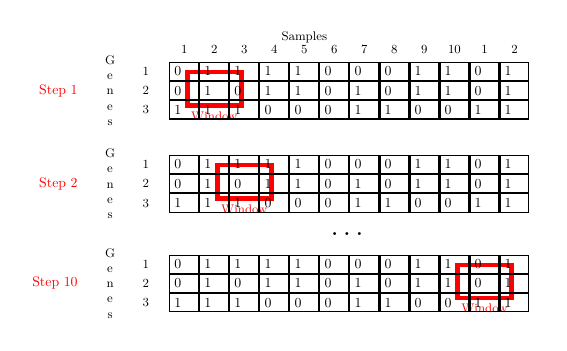
\begin{tikzpicture}[node distance=0.2cm,scale=0.5]

\matrix (data1)[matrix of nodes,nodes={draw,text width=0.5cm,scale=0.5}]
{
0 & 1 & 1 & 1 & 1 & 0 & 0 & 0 & 1 & 1 & 0 & 1\\
0 & 1 & 0 & 1 & 1 & 0 & 1 & 0 & 1 & 1 & 0 & 1\\
1 & 1 & 1 & 0 & 0 & 0 & 1 & 1 & 0 & 0 & 1 & 1\\
};
\matrix (data2)[below=of data1,matrix of nodes,nodes={draw,text width=0.5cm,scale=0.5}]
{
0 & 1 & 1 & 1 & 1 & 0 & 0 & 0 & 1 & 1 & 0 & 1\\
0 & 1 & 0 & 1 & 1 & 0 & 1 & 0 & 1 & 1 & 0 & 1\\
1 & 1 & 1 & 0 & 0 & 0 & 1 & 1 & 0 & 0 & 1 & 1\\
};
\node [below=of data2,yshift=0.2cm](p){\ldots};
\matrix (data10)[below=of p,matrix of nodes,nodes={draw,text width=0.5cm,scale=0.5},yshift=0.2cm]
{
0 & 1 & 1 & 1 & 1 & 0 & 0 & 0 & 1 & 1 & 0 & 1\\
0 & 1 & 0 & 1 & 1 & 0 & 1 & 0 & 1 & 1 & 0 & 1\\
1 & 1 & 1 & 0 & 0 & 0 & 1 & 1 & 0 & 0 & 1 & 1\\
};
\foreach \x in {1,...,10}
{
\node [above=of data1-1-\x,scale=0.5,yshift=-0.3cm] (sl\x) {\small{\x}};
}

\node [above=of data1-1-11,scale=0.5,yshift=-0.3cm] (sl11) {\small{1}};
\node [above=of data1-1-12,scale=0.5,yshift=-0.3cm] (sl12) {\small{2}};

\node [above=of sl5,scale=0.5,yshift=-0.6cm] {\small{Samples}};

\foreach \step in {1,2,10}
{
\foreach \x in {1,...,3}
{
\node [left=of data\step-\x-1,scale=0.5] (gl\x) {\small{\x}};
}
\node [left=of gl2,text width=10pt,text centered,scale=0.5] (geneslabel) {\small{G\\e\\n\\e\\s\\}};
\node [left=of geneslabel,red,scale=0.5] {Step \step};

\begin{pgfonlayer}{background}
\pgfmathadd{\step}{2}
\node [draw=red!100,fit=(data\step-1-\step)(data\step-3-\pgfmathresult),yshift=-1pt,ultra thick,scale=0.5] (win\step) {};
\node [below=of win\step,red,yshift=0.2cm,scale=0.5] {\small{Window}};
\end{pgfonlayer}
}
\end{tikzpicture}
\end{center}
 \caption{An example of shifting window for similarity analysis. Each position of the
windows is a step in the algorithm. At each step, expression levels of all samples in the window are compared
for each pair of genes. Window is shifter circularly.}\label{figure:window}
\end{figure}
\begin{table}
\begin{center}
 \caption{Results of the example similarity analysis carried on in
Figure~\ref{figure:window}}\label{table:exampleresult}
\begin{tabular}{|l|c|c|c|}
\hline
 & 1-2 & 1-3 & 2-3\\ \hline
Step 1 & + & + & - \\ %\hline
Step 2 & + & + & - \\ %\hline
Step 3 & + & - & - \\ %\hline
Step 4 & + & - & - \\ %\hline
Step 5 & + & - & + \\ %\hline
Step 6 & + & - & + \\ %\hline
Step 7 & + & - & - \\ %\hline
Step 8 & + & - & - \\
Step 9 & + & - & - \\
Step 10 & + & - & - \\ \hline\hline
Global & + & - & - \\ \hline
\end{tabular}
\end{center}
\end{table}

Figure \ref{figure:window} visualizes the search process with the sliding window. At each step, for each 
positioning of the window, local similarity measure between each pairs of genes are calculated as following:

\begin{equation}
\gamma^p(g_i,g_j) = \sum_{k=p}^{p +WS}
\begin{cases}
1 & \text{if} EL_k(g_i) = EL_k(g_j)\\
0 & \text{else}\\
\end{cases}
\end{equation}

\begin{equation}
SML^p(g_i,g_j) = \frac{\gamma^p(g_i,g_j)}{WS}
\end{equation}

Function $\gamma$ calculates the number of identical positions for a specific positioning of the window ( at 
$[p, p+ WS$])  where $WS$ is the window size and $EL_k(g)$ is the expression level of gene $g$ at sample 
$k$. Thus $SML$ function, calculating the frequency of samples with identical expression values for both genes,
 gives the local similarity measure between two genes for a specific positioning 
of the window. By using the $SML$ function, it is possible to calculate the similarity measure as following:

\begin{equation}
\delta(g_i,g_j)=\sum_{k=1}^{\# of samples} 
\begin{cases}
1 & \text{if} SML^k(g_i,g_j) > \theta_l \\
0 & \text{else}\\
\end{cases}
\end{equation}

\begin{equation}
SM(g_i,g_j) = \frac{\delta(g_i,g_j)}{\# of samples}
\end{equation}

Function $\delta$ calculates the number of window positionings where local similarity measure $SML$ 
exceeds a threshold $\theta_l$. Thus by calculating the frequency of local similarities exceeding this 
threshold value, we obtain similarity measure function $SM$ which maps a pair of genes to $[0,1]$.

Among the two threshold values used, the first one is called \emph{local similarity threshold}; it is used in
comparing the expression values of genes for a fixed placement of the window. This threshold determines how
strong we define the similarity concept for our purpose. When this threshold is low, for each placement of
the window, the expression levels of the two analyzed genes are marked similar more often. When this
threshold is high, the two analyzed genes have similar expression levels for a placement of the window only
when they follow exactly the same pattern.

The second threshold value is called \emph{global similarity threshold}; it is used in deciding whether two
genes are globally similar. This threshold determines the allowed degree of locality for observing the
similarity between two genes in order to mark them globally similar. When this threshold is high, the
similarity between the two genes should be observed in all the gene expression data (i.e., for all placements
of the window) for marking them similar. When this threshold is low, only local similarities might be
sufficient for marking the two genes similar.

In our experiments, we selected values for both thresholds empirically by running some initial tests and we
compared different values. In this work, for the gene expression data, it is important for us to have high
confidence in the similarity of the expression levels. And the gene expression data is known to have very
small number of samples. So, we always used very high values for both similarity thresholds, typically
over~75\%.

Another parameter used in the method is window size. The size of the window determines the number of samples
compared at each iteration of the algorithm. In a way, window size defines the locality. When the window size
is small, only a small number of samples are compared at each step. When the window size is large, a
significant portion of the whole data is compared for each step. Here it is worth noting that we are using a
twofold comparison scheme; first we compare all the values inside a sample and decide on local similarity;
and second we repeat this process by sliding the window through the data and accordingly decide on global
similarity. In the conducted experiments, we concluded that when both thresholds have similar values the
twofold process produces similar results for any choice of the window size. It is also possible for the
reader to grasp this result by considering the two extreme cases, where window size is~1 and windows size is
equal to the sample size, respectively.

When the window size is equal to~1, values for a single sample are compared at each step. Two genes are
marked as similar if they have the same expression level, regardless of the value of the local similarity
threshold (since there is a single sample, it is not possible to calculate a frequency). For deciding whether
two genes are similar globally, we test whether the frequency of the local similarity is higher than the
global similarity threshold. Consider two genes with expression data of $10110101$ and $01000110$. When the window size is equal to one, each position of the data produces a separate local similarity. And we decide whether they are similar or not, based on the global similarity threshold. If this threshold is 50\%, we mark these two genes as not similar since only 2 of 8 local similarity checks  succeed.

When the window size is equal to the sample size, there is a single step for testing local similarity, where
all samples are compared (the window surrounds the whole data). Two genes are marked as similar if the
frequency of the samples at which the two genes have the same expression level is larger than the local
similarity threshold. This process is not repeated and two genes are marked as globally similar if they are
locally~similar. Consider the same genes again with expression data of $10110101$ and $01000110$. When the window size is equal to 8, we determine local similarity based on the whole data. If the local similarity threshold is 60\%, then the whole data will not be marked as locally similar, since only 2 samples are equal. Since the only local similarity check does not succeed, two genes are marked as dissimilar.


Note that these two cases become identical in case the global similarity threshold and the local similarity
threshold are equivalent. In both cases, the two genes are similar if the frequency of samples with similar
expression levels for the two genes is above the threshold. This conclusion similarly follows for any window
size.

Since we are using a window to compare gene expression values locally, our approach is sensitive to the order of samples. The windows used is shifted through the data circularly and theoretically it is possible that two different orderings of the samples might produce different results for the analysis we carry on.

In this work, we assumed that the gene expression data is given in a specific ordering which  is treated as a problem parameter, where the sampling methods or strategy might have some meaning as in the case of time-series data. We do not attempt to reorder the samples, or consider different permutations of samples. We assume that the order in which the samples are given is better than any other alternative, unless we have prior knowledge. There are two reasons for this assumption. First, without any further knowledge on the correct ordering of data, it is only possible to consider all permutations of samples, which is a computationally intractable task. Second, especially in the case of real biological data we know that the original order of the data might have a real life impact on the dataset.

Note that the effect of ordering on analysis results is also related to the windows size. Consider expression data for two genes $10101010$ and $11111111$. For a window of size 1 and global similarity threshold 60\%, these two genes would be marked as dissimilar, since none of the local similarity test succeeds. For a window size of 4 with local similarity threshold of 60\% and global similarity thresholds 25\%, these genes would be marked dissimilar again. When we reorder the samples of the first gene as $11110000$, first analysis still produces the same result; however second analysis would mark the genes similar, since three of the local similarity tests succeed. Larger  windows decrease the coincidental positive or negative effects of ordering and leads to more accurate analysis results generally.

In experimental evaluation chapter we also present an independent study on the order of samples. This study also shows that preserving the original ordering of data does not seem to reduce the correctness of the analysis, on the contrary original ordering produces slightly more confident results than the average case.

We have also improved this simple comparison algorithm in order to deal with noise in the data, namely
shifted windows. For each window position, the comparison is actually performed multiple times, each time
shifting the expression data for one of the genes. The genes are labelled similar for the actual window
position if any of these comparisons succeeds. The improved version of the process is given as
Algorithm~\ref{algorithm:partition}.

{\small
\begin{algorithm}
\dontprintsemicolon
\KwIn{$m \times n$ gene expression data matrix $D$ ($m$ genes, $n$ samples), gene set $G$ ($m$ elements), window size $w$, window shift amount $s$, similarity threshold $\theta_l$, global similarity threshold $\theta_g$}
\KwResult{Similarity matrix $SM$, similarity list $SL$}
Initialize $SM$ to all zero \; \For(shift window through all samples circularly){$i = 0$ to $n - w$} {
    $wp_1 \longleftarrow [i, i+W]th$ columns in $D$ \;
    \ForEach {gene pair $g_1,g_2  (g_1 != g_2)$}{
        \For(shift one window){$j = -$$s$ to $s$}{
            $wp_2 \longleftarrow D [i+j, i+W+j]th$ columns in $D$ \;
            sim $\longleftarrow$ number of identical entries in $g_1^{th}$ row of $wp_1$ and $g_2^{th}$ row of $wp_2$ \;
            \If{sim $> \theta_l * w$}{
                $SM[g_1,g_2] += 1$ \;
                $SM[g_2,g_1] += 1$ \;
                \SetKw{Break}{break for}
                \Break\;
            }
        }
    }
} Divide all entries in $SM$ by $n$ \; \ForEach {gene pair $g_1,g_2  (g_1 != g_2)$}{
    \lIf{$SM[g_1,g_2] > \theta_g$}{add $(g_1,g_2)$ to $SL$}
} \caption{Gene Expression Data Analysis}~\label{algorithm:partition}
\end{algorithm}
}

The result of Algorithm~\ref{algorithm:partition} is used to serve two purposes in this work, namely
identifying classes of genes and constructing the transition function; details are discussed in the~sequel.

\section{Identifying Classes of Genes}
The similarity relation calculated in the previous subsection is used in our work for decomposing the
formulated POMDP problem into subproblems; each subproblem contains problem components closely related to
each other, but not coupled with other subproblems and other problem component.

For the GRN control problem, the similarity relation provides an appropriate way for guiding the
decomposition. In the POMDP formulation of the problem, the expression level of each gene is a state
variable, intervening and observing the expression level of each gene is a potential action and observation.
So it is possible to define each subproblem in terms of a set of genes. Each subproblem defined in this
fashion, is only related to the set of genes, as if these genes are closely coupled as a group; isolating
this group leads to isolate a part of the control problem.

The similarity relation introduced in the previous subsection is clearly an equivalence relation by
definition. Thus, the relation can be used to partition the gene set into classes. Each class is simply a set
of genes. Our aim is to define a POMDP subproblem for each class. In the classification process, we use the
similarity list produced by the gene expression data analysis. The process for constructing classes is
described in Algorithm~\ref{algorithm:analyze}. Chapter~\ref{chapter:decomposition} presents how subproblems are
created by using these classes.

{\small
\begin{algorithm} \dontprintsemicolon \KwIn{Similarity list SL, gene set $G$ ($m$ elements)}
\KwResult{$A$ partition of gene set $P$} $P \longleftarrow \emptyset$ \ForEach{gene $g$ in $G$}{
    \uIf{empty(P)} {
        $P \longleftarrow \{\{g\}\}$\;
    }
    \Else{
        \ForEach{class $c$ in $P$}{
            \lIf{SL contains $(g,g')$ for each $g' \in c$}{add $g$ to $c$}
        }
        \lIf{$g$ is not added to any class}{$P \longleftarrow P \bigcup \{\{g\}\}$}\;
    }
} \caption{Forming classes of genes}~\label{algorithm:analyze}
\end{algorithm}
}

\section{Constructing the Transition Function}
\label{section:transitionf} The similarity matrix produced from the gene expression data analysis is used in
the POMDP formulation of the GRN control problem. The entry at position ($i$,$j$) in the matrix is used as
the conditional probability value $Pr(gene_i = on | gene_j = on)$. This probability value is used for
constructing the transition function of the POMDP problem.

When constructing the transition function for the factored representation, we do not need a joint probability
distribution of state changes.  For each state variable~$s$, we need a probability distribution of the value
of the state variable, given values of other related states at the previous state of~$s$. By ``related
variables", we mean state variables that are known to influence the next value of~$s$.

For the GRN control problem, since each state variable is a gene, we need a probability distribution over the
expression level of a gene, given the expression levels of related genes. The ``related genes" can easily be
found by using the GRN.

{\small
\begin{table}
\begin{center}
\caption{An Example on Inferring Conditional Probabilities Between Genes}\label{geneitable}
\begin{tabular}{|c|c|c|c|}
  \hline
  % after \\: \hline or \cline{col1-col2} \cline{col3-col4} ...

  $gene_j$ & $gene_k$ & \multicolumn{2}{c|}{$gene_i$} \\ \cline{3-4}
    & & On & Off \\
    \hline
  On & On &  0.85 * 0.55 = 0.47 / 0.87 & 0.15 * 0.45 = 0.07 / 0.13 \\
  On & Off & 0.85 * 0.45 = 0.38 / 0.83 & 0.15 * 0.55 = 0.08 / 0.17 \\
  Off & On & 0.15 * 0.55 = 0.08 / 0.17 & 0.85 * 0.45 = 0.38 / 0.83 \\
  Off & Off & 0.15 * 0.45 = 0.07 / 0.13 & 0.85 * 0.55 = 0.47 / 0.87 \\
  \hline
\end{tabular}
\end{center}
\end{table}
}


For constructing the probability distributions, we assumed that the relationship between two genes is
always independent of the other relationships. Thus, if a gene is influenced by multiple genes, each
interaction is considered as an independent event. This assumption simplifies the calculation of the
transition function.Also we assumed that genes behave according to a linear model. Thus a
gene only effects other genes positively or negatively and the effected gene is influenced by
a linear combination of all influences.

Our transition function formulation has two steps:

\begin{enumerate}
\item Gene expression data is analyzed and similarity on the behavior of genes is extracted. Details 
of this analysis is presented in Section \ref{section:dataanalysis}. The output of this analysis step 
is a function $SM$ defined $G \times G \to [0,1]$ where $G$ is the set of genes in GRN. This function 
represent the similarity of any two genes, where value 1 indicates two genes behave identically for the
data we analyzed.

\item We use the similarity measure function $SM$ produced at the previous step and the GRN to formulate 
the transition function of the POMDP model. We make use of the factored representation in this step 
to simplify the process. Each gene is conceived as a state variable and the transition function is calculated 
for each gene separately.

We assume that only a limited number of other genes directly effect the expression level of a gene. 
This assumption is also used in PBN model, where each node is connected to only a limited number of 
other nodes. For determining which genes effect a given gene directly, we refer to the gene regulatory
network. A gene $g_i$ is assumed to be directly influenced by another gene $g_j$ if there is a directed
edge $(g_j,g_i)$ in the gene regulatory network.

Assume that for each gene $g_i$, the gene is influenced by only genes $g_i ^1, g_i^2,... g_i^j$
directly. Then we formulate factored transition function $T$ that determines the expression level of 
gene $g_i$ at next time step, given expression levels of genes  $g_i ^1, g_i^2,... g_i^j$ by using 
probabilities:
\begin{multline}
Pr(g_i = on , g_i ^1, g_i^2,... g_i^j ) = \\
 \prod_{x = 1}^j 
\begin{cases}
SM(g_i,g_i^x) & \text{if } g_j^x = on,\\
1 - SM(g_i,g_i^x) & \text{if } g_j^x = off.
\end{cases}
\end{multline}
\begin{multline}
Pr(g_i = off , g_i ^1, g_i^2,... g_i^j ) = \\
\prod_{x = 1}^j 
\begin{cases}
SM(g_i,g_i^x) & \text{if } g_j^x = off,\\
1 - SM(g_i,g_i^x) & \text{if } g_j^x = on.
\end{cases}
\end{multline}

For factored representation, the state space is expressed in terms of each state variable seperately. 
Thus it is possible to directly use these probability values as descriptors of 
state variables. The POMDP planer will take care of calculating the plain transition function where
necessary.

It is possible to formalize this function in the plain POMDP notation equivalently. One need to calculate
joint probability values by assuming that each probability calculated is independent of each other. This 
assumption is compatible with our previous assumption, where each gene is only influenced by genes it is 
connected to in th GRN.

Calculating joint transition probabilities by using these values gives us the transition function with no 
intervention action \emph{noop} performed (such as $T'(s,s')$ that does not depend to any action. 
If $A$ is the action function over $S \to S$ we can derive $T$ for other actions as:

\begin{equation}
T(s,noop,s') = T'(s,s')
\end{equation}
\begin{equation}
T(s,a,s') = T'(A(s),s')
\end{equation}
\end{enumerate}

As we stated before, since we use the factored POMDP representation, our formulation only need to express
transition probabilities for each gene and action descriptions. When action descriptions and state transitions 
are given together, plain representation of the state transition function can easily be generated by the planner.


To illustrate the process, assume gene $i$ is influenced by genes $j$ and~$k$. The
similarity matrix contains the values $SM(j, i) = 0.85$ and $SM(k, i) = 0.55$. Then the conditional
probability distribution of gene $i$ is computed as given in Table~\ref{geneitable}.

Also gene expression levels do not change instantly; we assumed that the expression level of each gene
depends on the expression level of the previous state. To reflect this, all the probabilities are multiplied
by~0.9 on the condition that the expression level does not change, and they are multiplied by 0.1 on the
condition that the expression level changes. For example, the value 0.47 that reflects $Pr(gene_i^t = On |
gene_j^{t-1} = On, gene_k^{t-1} = On)$ is further refined as $Pr(gene_i^t = On | gene_j^{t-1} = On,
gene_k^{t-1} = On, gene_i^{t-1} = On) = 0.9 \times 0.47 = 0.42$ and $Pr(gene_i^t = On | gene_j^{t-1} = On,
gene_k^{t-1} = On, gene_i^{t-1} = Off) = 0.1 \times 0.47 = 0.04$.

Note that these values are not actual probability distribution. We need to normalize these values in order to
use them as transition probabilities. The values shown after the / in Table \ref{geneitable} are normalized values. Note that values in a row add up to 1.

\newpage

\chapter{POMDP Decomposition}
\label{chapter:decomposition}

 The previous chapters presented the POMDP problem formulation of the GRN control
problem. As we have stated above, after this formulation, it is possible to use any POMDP solver to generate
a policy and intervene with the GRN accordingly. In order to efficiently solve the POMDP problem, we also
developed a method to pre-process the POMDP problem. The goal of this method is decomposing the POMDP problem
into subproblem. Each subproblem will contain genes closely related and exhibiting similar behavior. The
motivation behind this decomposition is separating different parts of the problem from each other.

One of the important problems of the existing POMDP solution methods is curse of
dimensionality~\cite{Bellman61}. The complexity of solving the problem is dominated by the number of possible
states and for a flat representation, POMDP problems have huge state space (exponential in terms of state
variables). Fortunately, factored representation is a way to represent the problem in a more compact form.
However, without taking advantage from this compact representation, the computational cost of the solution
methods does not decrease. Decomposing the problem into subproblems produces a number of subproblems; each
subproblem can be solved with a very small computational cost compared to the cost of solving complete large
problem. Moreover, separating different parts of the problem provides the chance to identify and remove the
unrelated subproblems from the solution process.

The gene expression data analysis explained in Section~\ref{section:dataanalysis} is the method we used for
identifying classes of genes. The next subsections present how the subproblems are created for each class and
how these subproblems are coordinated for the~solution.  Algorithm \ref{algorithm:decompose} gives a brief outline
of POMDP decomposition.

{\small
\begin{algorithm}
\dontprintsemicolon
\KwIn{M: POMDP Problem Formulation of GRN Control Task, G: Gene Regulatory Network, P: Partitioning of genes }
\ForEach{partition p in P}{Formulate pomdp problem for p using M   and add it to DEC-POMDP\;}
Eliminate Redundant Subproblems in DEC-POMDP\;
\ForEach{problem dp in DEC-POMDP}{
Determine Goal Description of dp\;
Postulate Action Set of dp\;
}
Construct Execution Graph EG using DEC-POMDP\;
Solve subproblems in DEC-POMDP\;
Execute Policy using solutions of DEC-POMDP and EG
\caption{POMDP Decomposition and Execution}~\label{algorithm:decompose}
\end{algorithm}
}

\subsection{POMDP Formulation of subproblems}

It is possible to apply the POMDP formulation presented in Chapter~\ref{chapter:formulation} to each
class of genes in order to produce POMDP formulation for the subproblems. However, we did not apply the same
method, instead we partitioned the POMDP problem into subproblems by using some elements of the POMDP
formulation in the process.

The main motivation for not using the same POMDP formulation as a constructive manner is the fact that the
main problem is something more than the union of the subproblems. It is possible to use the POMDP formulation
for constructing every component of every subproblem. However, some of the subproblems may contain genes that are influenced by genes that belong to other subproblems. Similarly, some of the subproblems may contain genes that influence genes that belong to other subproblems. We call these relations \emph{dependencies} and these dependencies are not components of any single subproblem. If we use this approach, we
should also regenerate these dependencies by repeating some of the steps used in constructing the main
problem. Moreover, generating components of the subproblems (e.g., transition functions) also require
multiple repetition of the already carried POMDP formulation. So, using the POMDP formulation for subproblems
brings a lot of excessive computation if we want the subproblems to fully express the main problem. Thus,
instead of repeating the same process, we adapted a decomposition approach which basically uses projections
or subsets of POMDP components of the main~problem.

Another motivation underlying not using the POMDP formulation is to keep the formulation and solving methods
independent from each other as much as possible. In this work, POMDP formulation and POMDP solving methods
have only a single common element, which is the gene expression data analysis. The POMDP solving method can
be adapted to any other partially observable probabilistic control problem by replacing the gene expression
data analysis with an appropriate method particular to the investigated problem (possibly a similar data
analysis component). However, if we had used the POMDP formulation for defining the subproblems, the solving
method would have been dependent on the POMDP problem formulation, which would have been customized for the
GRN control problem. This would severely affect the portability of the POMDP solving method.

In order to partition a POMDP problem, it is sufficient to partition each problem element. Partitioning the
state space, action space, observation space and observation function are trivial, since all of them are made
up of elements related to a single gene. For each existing partition, we identify the states, actions and
observations related to the genes in the partition. For each observation, the function can be defined based
on the same genes and by obeying the specifications given in Section~\ref{section:observation}.

The reward function for each subproblem is the same as the reward function defined for the main problem,
however the goal description might change. The goal of the main problem mentions a number of genes. For each
subproblem, we modify the goal description, such that it only mentions genes (i.e., state variables) related
to the subproblem.

Note that, some of the subproblems might not be related to any gene (state variable) mentioned in the goal
description. Thus, their goal descriptions become empty and the reward function becomes meaningless after
decomposition. Similarly, some of the subproblems might not be related to any input gene. Thus, these
subproblems would not contain any action after decomposition. We will enumerate and process these cases
further when coordinating the subproblems in the next~section.

The transition function is derived as explained in Section~\ref{section:transitionf}. The conditional
probability values extracted from the gene expression data are used for constructing the transition function
for each subproblem. However, for each subproblem, the transition function only contains probability
distributions for expression levels of related genes.

Note that a gene $g$ might be influenced by gene $g'$ from another partition. In this case, the similarity
value between the two genes should be used when constructing the transition function. However, using this
dependency in the transition functions of both subproblems is redundant. We only add the influenced gene
($g$) to the subproblem containing influencing gene ($g'$), and we use the similarity value to calculate the
transition function value regarding $g$ and $g'$. Influenced gene ($g$), which now exists in both
subproblems, is called \emph{subproblem input} for the original subproblem in which it exists; and it is
called \emph{subproblem output} for the other subproblem to which it is added.

This is the outline for producing each subproblem from the main POMDP problem components and gene expression
data analysis. When all the subproblems are constructed, what is left is to postprocess them in order to fill
any remaining detail in their formulation, and coordinating the subproblems to produce a policy for the main
problem.

\subsection{Coordinating Subproblems}
\subsubsection{Idea Behind Coordination}
By decomposing the POMDP problem, we obtained a number of subproblems. It is possible to solve these problems
by a POMDP solver; however, we need to organize the solution process by coordinating these subproblems. The
idea behind this organization is to establish how each subproblem contributes to the main problem. Each
subproblem contains three kinds of genes (or state variables in a more general form):

\begin{enumerate}
  \item \textbf{Influencing Genes:} It is possible to influence the expression levels of these genes. This group contains:
  \begin{enumerate}
    \item \textbf{Input genes:} These are genes that are in the input gene set of the main control problem
    \item \textbf{Subproblem input genes:} These are genes that are not in the input gene set of the main control problem
    (i.e., can not be influenced directly), however their expression level is influenced by gene(s) that belong to another subproblem.
  \end{enumerate}
  \item \textbf{Influenced Genes:} The expression levels of the genes in this group are important because this group
  contains:
  \begin{enumerate}
    \item \textbf{Target genes:} These are genes that are in the target gene set of the main problem
    \item \textbf{Subproblem output genes:} These are genes that are not in the target gene set, however their expression
    levels influence gene(s) that belong to another subproblem.
  \end{enumerate}
  \item \textbf{Abstract Genes:} It is not possible to influence the expression levels of these genes, and furthermore
  their expression levels are not important because they are neither influencing nor influenced genes.
\end{enumerate}

Note that a gene can be a member of more than one group. For example, an input gene might also be a subproblem output gene.

Each subproblem can be viewed as a small portion of the main control problem. Each subproblem has two
purposes:
\begin{enumerate}
  \item If all of the subproblems have little or no dependency (i.e., there is only a small number of subproblem
  input and output genes) then solving each subproblem is enough for deducing a policy to control target genes that
  belong to this subproblem. In this case, we can see each subproblem as a portion of the main control
  problem; it is concentrated on a group of target genes and all unrelated problem elements are discarded.
  \item If subproblems have dependencies among themselves, beside solving each subproblem for controlling target
  genes, we should also take into consideration effects of each subproblem on others. Subproblem input and output
  genes are formulated for this purpose. They maintain the dependencies between subproblems and can be used for
  controlling how one subproblem influences another.
\end{enumerate}

By solving subproblems it is possible to control the influenced genes, which contains target genes and subproblem output genes. Controlling target genes is the main purpose, and controlling subproblem output genes allows us to control subproblem input genes. Subproblem input genes, with input genes, are used as control inputs of the sub problems when solving them. Abstract genes acts as hidden state elements that effect the system dynamics, but can not be controlled directly and their expression values are not important for our purposes.

As an example. assume a gene regulatory network of genes labelled from 1 to 8 as shown in Figure \ref{figure:grn1}. Genes 1, 2, 3, 4, and 5 are observable. Genes 1 is input genes and gene 2 is the target gene. Assume a subproblem set generated by our approach is $\{\{1,3\},\{2,4,8\},\{5,6,7\}\}$. For the first subproblem, gene 1 is both an input gene and a subproblem output gene; gene 3 is a subproblem output gene. For the second subproblem genes 4 and 8 are subproblem input genes since all of them are influenced by gene 1;  gene 2 is a target gene. For the third subproblem gene 5 is influenced by gene 3; genes 6 and  7 are influenced by gene 1 so all of them are subproblem input genes.

\subsubsection{Eliminating Redundant Subproblems}
The first step in coordinating the subproblems is to decide for each subproblem, whether we should solve it
or not. It is obvious that we should solve the subproblems with a goal description (i.e., subproblems related
to at least one of the target genes). However, we mentioned before that some of the subproblems might not
have a goal description (i.e., not related to any of the target genes). We should decide which one of them
should be solved.

We use a simple algorithm for this purpose. First, we mark all subproblems with a goal description to be
solved. Then, we iterate over the remaining subproblems. If any of these subproblems contain a subproblem
output which is related to a subproblem previously marked ``to be solved'', then the subproblem containing
the output is also marked ``to be solved''. We repeat this iteration until no more subproblem could be marked
``to be solved''.

By using this simple algorithm, we identify all subproblems directly or indirectly related to the controlling
target genes. It is sufficient to solve only these subproblems and the other subproblems are discarded.

Note that there is a slight possibility that subproblems marked ``to be solved'' do not contain any of the
input genes. In this case, we can conclude that the input genes are not influential on the target genes and
the control problem has no possible solution, regardless of the formulation used.

Considering the example of the previous subsection, subproblem $\{5,6,7\}$ can safely be eliminated since all subproblem input genes of the subproblem $\{2,4,8\}$ are related to subproblem $\{1,3\}$ and this subproblem does not have any subproblem inputs.

\subsubsection{Determining Goal Descriptions}
For the second step, we should formulate goal descriptions for subproblems marked ``to be solved''. It is
guaranteed that these subproblems have subproblem outputs (If they did not have, then either they would not
be marked ``to be solved'', or they would already have a goal description). The outputs of these subproblems
should be used as goal description. However, it is not possible to automatically specify whether it is
desirable for these genes to be expressed or not.And also there is a non-trivial relationship between these subproblem output genes and related subproblem input genes. In order to postulate a complete problem description, we add the related subproblem input genes to the problem and mark them as goal of the subproblem. However,  it is still not possible to state whether it is desirable for these genes to be satisfied, or not. Thus, we produce multiple copies of these subproblems, one
for each expression level of the goal genes. If there are $k$ goal genes for a given
subproblem, we produce $2^k$ copies of the problem, assuming a binary expression level. In the worst case,
this approach produces exponential number of copies of each problem and the total performance of the method
suffers from this step. However, for most cases, if the gene expression data properly partitions the genes,
then each subproblem would have very few number of (typically 1 or 2) goal genes. Thus, we predict
that this approach will on average contribute a constant factor to the computational complexity.

Continuing with our example, for the first subproblem ${1,3}$ we extend the problem to ${1,3,4,8}$ and the goal description includes genes 4 and 8. For the second subproblem, goal description only includes gene 2. This means we have to solve 4 copies of problem 1 for each possible goal description regarding genes 4 and 8; we only need to solve a single copy of the second subproblem.

\subsubsection{Postulating Action Sets}
For the third step, we formulate actions for all subproblems. We have already mentioned above that some of
the subproblems might not contain any action at all. If these subproblems contain subproblem inputs, these
genes are treated as input genes and action descriptions for controlling these genes are provided. If these
subproblems do not contain any input gene or subproblem input, then they are discarded and marked as ``not to
be solved''. We repeat this process until no subproblem is discarded.

Note that there is also a slight possibility that the subproblems discarded in this step contain target
genes. In this case, we can conclude that these target genes can not be controlled by any input gene. If all
of the target genes are removed in this fashion, we can conclude that the problem has no possible solution,
regardless of the formulation used.

For our example since both subproblems contains input genes or subproblem input genes, none of them can be eliminated. Action set for the subproblem $\{1,3,4,8\}$ only contains gene 1; action set of subproblem $\{2,4,8\}$ contains genes 4 and 8.

\subsubsection{Construction of Execution Graph}
For the fourth step, we construct a directed graph of subproblems. Vertices of the graph are subproblems and
there is a directed edge between two subproblems connected with a subproblem input-output pair. This graph
structure is our scheme for solving subproblems. For simplicity, we process this graph and remove all loops.
We detect loops from short to longer, and for each loop found, all subproblems in the loop are merged into a
single problem. The merging process can be carried out as the inverse of decomposition. State, action, and
observation spaces are merged; observation functions are merged; new reward functions and transition
functions are formulated. Finally, as a binding element, all subproblems on the directed graph are solved
using POMDP solver. Each subproblem generates a policy for intervening its input genes. Note that these input
genes might be actual input genes, or subproblem inputs. The policy elements with actions intervening actual
input genes can be realized; however, it is not possible to realize the policy elements with actions
intervening subproblem inputs. So, we apply a controlled execution scheme.

We select the subproblems with target genes as main execution subproblems. At each instance, the policies
generated by these subproblems are always executed. For input genes related to these subproblems, intervening
actions are executed directly. However, for actions intervening subproblem inputs, we do not execute any
action; we just select the related subproblem's policy for execution. For example, assume that $SP_a$ is a
subproblem containing a target gene as state variable and gene $i$ as subproblem input. There exists another
subproblem $SP_b$ with subproblem output gene $i$ (there should be an edge in the binding graph from $SP_b$
to $SP_a$). Then if the policy generated by $SP_a$ tells us to intervene with gene $i$ and set its expression
level to $on$, then we execute the policy related to $SP_b$. At each instance, we can just select the
policies to be executed in this fashion. Since each subproblem contains different genes and different action,
no inconsistency arises from executing multiple policies.

For our example, the execution graph is a simple 2-node graph. There is a directed edge from subproblem $\{1,3,4,8\}$ to subproblem $\{2,4,8\}$. Execution is based on subproblem $\{2,4,8\}$. Genes 4 and 8 are input to this subproblem. A policy is based on these input genes. Four copies of subproblem $\{1,3,4,8\}$ are solved for each possible expression level of genes 4 and 8. Whenever the policy for the subproblem $\{2,4,8\}$ requires genes 4 and 8 are set to specific expression levels, the related policy is fetched and input gene $1$ is set to the expression level designated in the fetched policy.

\newpage

\section{Experimental Results}
\label{chapter:experiments}

MOD* Lite is a domain independent algorithm and can be applied to any virtual environment with given $n$ objectives. These objectives could be whether \textit{maximized} or \textit{minimized}. The vital assumption about objectives is their independence from each other. If two objectives could effect each other in a positive or negative manner, this might reduce or expand objectives vector size, which is out of this work's scope. Thus, we assume that each defined objective is considered in different perspective and can not be transferred to each other.

The algorithm is tested on various environments with different scenarios. However, as it is not possible to exemplify all possible cases, specific and several extreme conditions are selected for experiments. MOD* Lite is compared with MOA* that guarantees optimal solutions in fully observable multi objective environments and MOGPP, a classic genetic solution which can be used for finding paths with multi objective cases.

For testing, all algorithms are implemented in Java language and run under Linux environment which has Intel(R) Core(TM) i7-2600 CPU @ 3.40GHz and 8 GB of RAM with -Xmx6192m parameter for JVM.

All tests are done on 2-D grid maps as detailed in Subsection \ref{envProperties}. In these tests, the agent tries to find available non-dominated best paths with respect to two objectives, path length and risk taken from threat zones. Thus, the agent endeavours to minimize both objectives and tries to find \textit{shortest} and \textit{safest} paths.

For all test cases, several parameters of MOGPP algorithm must be tuned. For instance; number of elitist individuals are $5$, population count and maximum iteration are $50$, and cross-over and mutation ratios are taken as $0.8$ and $0.05$, respectively. As MOGPP constructs initial paths randomly, each execution of the algorithm might not give exactly same results at the same execution time even the maps are equal. Thus, all given execution times and selected paths are considered as the average of 10 different executions for MOGPP.

\subsection{Fully Observable Tests}

First of all, it must be shown that MOD* Lite is complete and gives optimal and/or sub-optimal results in fully observable environments. The performance comparison is done in two dimensions, execution times and paths they generate (path quality), respectively.

In the first set of tests, randomly generated fully observable maps with different sizes (20 x 20, 40 x 40, 60 x 60, 80 x 80, 100 x 100, 120 x 120, 140 x 140 and 160 x 160), are used. Each of these maps have nearly 25\%-30\% percent threat zone and 14\%-16\% percent obstacle ratio. Agent's initial and target locations are taken as farmost cells on diagonal. For this case, execution times and generated paths' costs for different sized maps are given in Figure \ref{fig:rand_fully} and Table \ref{table:randPaths}. As seen from path qualities, MOA* finds optimal results and MOD* Lite finds optimal and/or sub-optimal results while gradually increases on the computation time manner. Although MOGPP works on similar times with MOD* Lite, it fails to find optimal or sub-optimal paths  especially for large scaled maps. One could set maximum iteration and population count to larger numbers to converge path quality to optimality, but this case increases execution time exponentially. Thus, more modest parameters are chosen for MOGPP to enforce the algorithm to yield reasonable results within expected time. 
 
Notice that taken risk values depend on environmental properties and should not be compared between different sized maps.

\begin{figure}
\centering
\includegraphics[width=2.5in, angle=270]{experimental/randomized_normal}
\caption{Execution Times of Randomly Generated Fully Observable Maps}
\label{fig:rand_fully}
\end{figure}

\begin{table}[ht]
	\caption{Non-dominated Path Costs For Randomized Maps}
	\centering
    \begin{tabular}{l l l l}
        \hline
        Map Size	&  MOD* Lite	&	MOA*		&	MOGPP \\ [0.5ex] \hline
        20 x 20		&	(39,90)		&	(39,90)		&	(41,916)
		   \cr		&	(43,0)		&	(43,0)		&	(43,408)\\
		   \\ 
        40 x 40		&	(79,9)		&	(79,9)		&	(89,2789)
		   \cr		&	(81,0)		&	(81,0)		&	(103,1239)
		   \cr		&				&				&	(105,296)\\
		   \\
		60 x 60		& 	(119,0)		&	(119,0)		&	(151,1970)
		   \cr		&				&				&	(169,549)
		   \cr		&			  	&				&	(181,426)\\
		   \\
        80 x 80		& 	(159,198)	&	(159,58)	&	(213,6382)
		   \cr		& 	(161,0)		&	(161,0)		&	(237,2007)
		   \cr		& 				&				& 	(263,1581)
		   \cr		& 				&				& 	(269,955)
		   \cr		& 				&				& 	(285,942)\\
		   \\
        100 x 100	&	(199,885)	&	(199,885)	&	(285,15804)	
		   \cr    	&	(201,708)	&	(201,708)	&	(295,14130)
		   \cr    	&	(203,0)		&	(203,0)		&	(299,14099)
		   \cr	  	& 				&				&	(305,10979)
		   \cr	  	& 				&				&	(341,9851)
		   \cr	  	& 				&				&	(377,177)\\		   
		   \\
        120 x 120	&	(239,0)		&	(238,0)		&	(371,12817)
		   \cr		&				&				&	(399,7346)\\
		   \\
        140 x 140	&	(279,45)	&	(279,45)	&	(445,10920)
		   \cr		&	(281,42)	&	(285,12)	&	(483,5281)        
    	   \cr		&				&	(303,0)		&	(515,4000)
 		   \cr		&				&			 	&	(517,3520)\\
 		   \\
        160 x 160	&	(319,0)		&	(319,0)		&	(545,7530)
		   \cr		& 			 	&			 	&	(547,4602)\\ [1ex]
        \hline
    \end{tabular}
	\label{table:randPaths}
\end{table}

In the second set of tests, each algorithm is executed on handcrafted maps with same sizes, threat zone and obstacle ratio with randomized tests as indicated in previous test case. These maps are also assumed fully observable and agent's initial and target locations are as farmost cells on diagonal. All handcrafted test environments \textit{guarantee} that at least two non-dominated paths will be available. Execution times are shown in Figure \ref{fig:hand_fully} and generated paths' costs are given in Table \ref{table:handPaths}.

\begin{figure}
\centering
\includegraphics[width=2.5in, angle=270]{experimental/handcrafted_normal}
\caption{Execution Times of Handcrafted Fully Observable Maps}
\label{fig:hand_fully}
\end{figure}

\begin{table}[ht]
	\caption{Non-dominated Path Costs For Handcrafted Maps}
	\centering
    \begin{tabular}{l l l l}
        \hline
        Map Size  &  MOD* Lite  & 	 MOA*  		&  	MOGPP\\ [0.5ex] \hline
        20 x 20   &	(39,264)	&	(39,264)	&	(39,1614)
		   \cr    &	(41,258)	&	(43,6)		&	(41,394)
   		   \cr    &	(45,0)		&	(45,0)		&	(47,264)
   		   \cr	  &				&				&	(49,0)\\ 
   		   \\
        40 x 40   & (79,528)	&	(79,528)	&	(95,1637)
		   \cr	  &	(81,352)	&	(81,352)	&	(115,880)
		   \cr	  &	(91,156)	&	(91,156)	&  
		   \cr	  &	(97,0)		&	(97,0)		& \\
		   \\
        60 x 60   & (119,243)	&	(119,243)	&	(159,4761)
		   \cr	  & (123,33)	&	(123,33)	&	(165,1979)
   		   \cr	  & (127,0)		&	(127,0)		&	(167,165)
   		   \cr	  &				&				&	(233,99)\\ 
   		   \\
        80 x 80   & (159,129)	&	(159,129)	&	(223,2327)
		   \cr	  &	(161,69)	&	(161,69)	&	(291,1627)
		   \cr	  &	(163,0)		&	(163,0)		& \\
		   \\
        100 x 100 &	(199,30)	&	(199,30)	&	(311,4827)
		   \cr	  &	(201,6)		&	(201,6)		&	(327,3042)
		   \cr	  &	(203,0)		&	(203,0)		&	(341,1989)
   		   \cr	  &				&				&	(353,45)
   		   \cr	  &				&				&	(365,0)\\ 
   		   \\
        120 x 120 & (239,77)	&	(239,77)	&	(363,11340)
		   \cr	  & (241,44)	&	(241,44)	&	(413,8821)
		   \cr	  &			   	&	(261,0)		&	(417,4613)		   
		   \cr	  &			   	&				&	(455,3830)
		   \cr	  &			   	&				&	(517,1292)\\
		   \\
        140 x 140 & (210,1774)	&	(210,1774)	&	(306,16134)
           \cr	  & (212,1728)	&	(212,1344)	&	(336,10836)           
   		   \cr	  & (214,40)	&	(214,40)	&	(368,6510)
		   \cr	  &	(244,0)	   	&	(244,0)		&	(390,4876) 
		   \cr	  &			   	&				&	(500,3335)   
		   \cr	  &			   	&				&	(514,2328)\\
		   \\
        160 x 160 & (319,913)	&	(319,601)	&	(497,41016)
           \cr	  & (321,581)	&	(321,354)	&	(563,19675)
   		   \cr	  & (323,0)		&	(323,0)		&	(719,14811)
		   \cr	  &			   	&				&	(859,9448)\\ [1ex]
        \hline
    \end{tabular}
	\label{table:handPaths}
\end{table}

In execution times in Figure \ref{fig:hand_fully}, it can be seen that MOGPP increases gradually instead of an exponential growth especially on large scaled maps. However, its path quality is not good enough when compared to MOD* Lite and MOA*' s results.

There exists a remarkable point that MOA* has nearly similar results with MOD* Lite in path quality manner. This case shows that even MOD* Lite is based on partially observable dynamic environments, it could also give \textit{as good results as} MOA* on stationary and fully observable environments and can be applied on those environments.

\subsection{Partially Observable Tests}

As discussed in previous sections; the main difference of MOD* Lite from existing classic path planning or evolutionary based algorithms is its adaptivity to partially observable dynamic environments. To show this advantage, partially observable tests are done with randomized maps of sizes 60 x 60, 80 x 80, 100 x 100 and 120 x 120. On these maps, agent's initial and target locations are chosen to be the furthermost cells in the environment. For each map, agent' s sensor range was set between 10\% to 60\% and execution times were observed. An example search space of MOD* Lite with 30\% sensor range can be seen in Figure \ref{fig:initialSearch}. In this figure, agent is depicted with a cyan dot. The fogged gray area represents agent' s sensor range and drawn purple path through temporary goal (blue dot) can be seen.

\begin{figure}
\centering
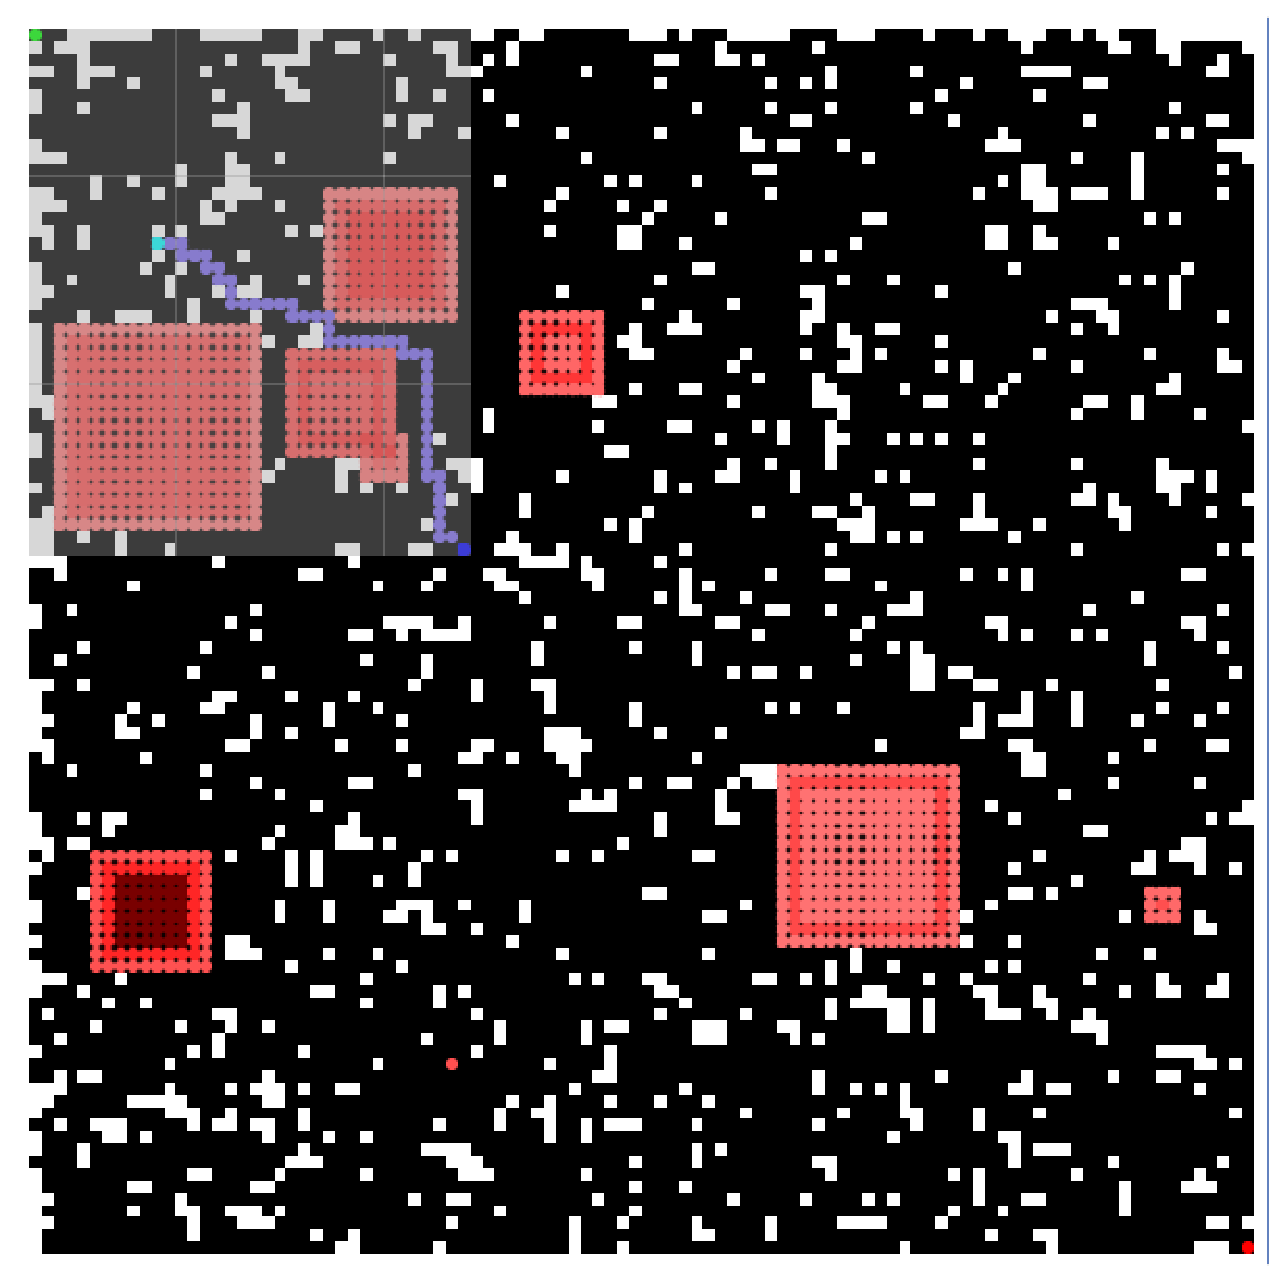
\includegraphics[width=2.5in, angle=270]{experimental/initialSearch}
\caption{A 100x100 Partially Observable Map with 30\% Sensor Range}
\label{fig:initialSearch}
\end{figure}

In these tests, the agent starts to plan a path towards the nearest available cell within its sensor range -the temporary goal- to the actual goal with respect to Manhattan Distance. After planning, consider that agent has found three paths with costs $(15, 200)$, $(18, 230)$ and $(23, 260)$. In such cases, the agent tends to choose the path with cost $(18, 230)$, the median of paths. This ad-hoc strategy could be set explicitly according to the domain that the algorithm works on. Afterwards, it starts to follow the chosen path. When new cells are available or a weight of a cell is changed within sensor range, agent reassigns the temporary goal and re-executes the path planner algorithm. This process iterates until the agent reaches to the desired goal location.

\begin{figure}
\centering
\includegraphics[width=2.5in, angle=270]{experimental/60x60_partially_normal}
\caption{60x60 Partially Observable Map on Different Sensor Ranges}
\label{fig:60x60sensor}
\end{figure}

\begin{figure}
\centering
\includegraphics[width=2.5in, angle=270]{experimental/80x80_partially_normal}
\caption{80x80 Partially Observable Map on Different Sensor Ranges}
\label{fig:80x80sensor}
\end{figure}

\begin{figure}
\centering
\includegraphics[width=2.5in, angle=270]{experimental/100x100_partially_normal}
\caption{100x100 Partially Observable Map on Different Sensor Ranges}
\label{fig:100x100sensor}
\end{figure}

\begin{figure}
\centering
\includegraphics[width=2.5in, angle=270]{experimental/120x120_partially_normal}
\caption{120x120 Partially Observable Map on Different Sensor Ranges}
\label{fig:120x120sensor}
\end{figure}

\begin{figure}
\centering
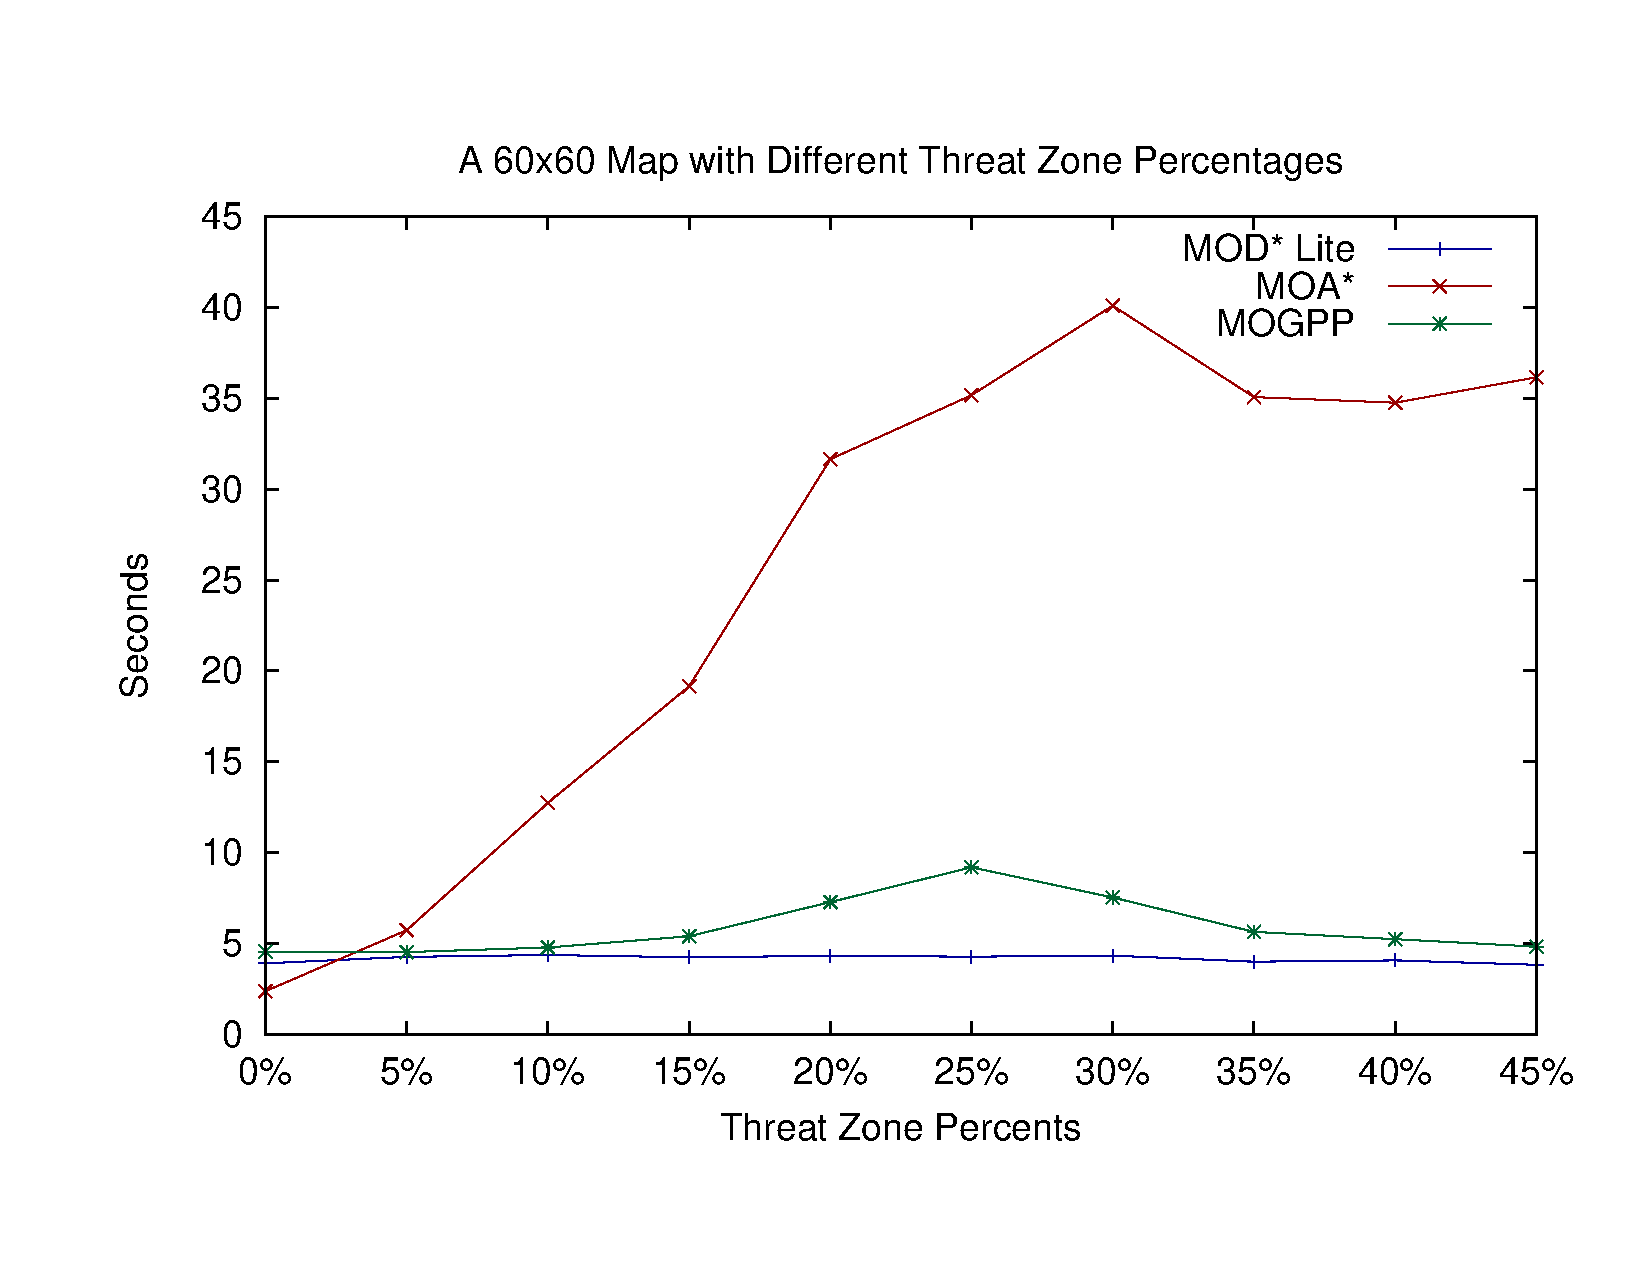
\includegraphics[width=2.5in, angle=270]{experimental/60x60_multiobj_normal}
\caption{Execution times of 60x60 Fully Observable Map on Different Threat Zone Percents}
\label{fig:tzratio60}
\end{figure}

\begin{figure}
\centering
\includegraphics[width=2.5in, angle=270]{experimental/80x80_multiobj_normal}
\caption{Execution times of 80x80 Fully Observable Map on Different Threat Zone Percents}
\label{fig:tzratio80}
\end{figure}

%\begin{table}[ht]
%	\caption{MOGPP Execution Times on a 125x125 Partially Observable Map}
%	\centering
%    \begin{tabular}{l l}
%        \hline
%        Sensor Range	&	Execution Time (sec.)\\ [0.5ex] \hline
%        20\%			&	402.325\\
%        30\%			&	420.481\\
%		40\%			&	1024.237\\
%		50\%			&	1351.854\\
%		60\%			&	1922.415\\ [1ex]
%        \hline
%    \end{tabular}
%	\label{table:mogpp125vFrustum}
%\end{table}

The fundamental advantage of MOD* Lite can be seen very clearly on these tests. While MOD* Lite has the capability of updating only the effected states due to its incremental nature, MOA* re-plans the overall path from scratch when new parts become known and the weights of some cells have changed. This situation causes MOA* and MOGPP to work on exponentially long times. Total execution times to reach to the target for these test cases are given in Figures \ref{fig:60x60sensor}, \ref{fig:80x80sensor}, \ref{fig:100x100sensor} and \ref{fig:120x120sensor}. As can be seen from results, MOD* Lite can easily handle the dynamical issues of the environment where MOA* and MOGPP fails. Due to discovering different parts of the environment during execution, actual traversed path's costs of MOD* Lite, MOA* and MOGPP might be slightly different from each other, where MOD* Lite could follow a better path with respect to MOA* or MOGPP or vice versa.

\subsection{Multi Objectivity Tests}

As threat zones and their risk values are used as the second objective, percentages of these zones also effect execution time and generated path quality. In this set of tests different threat zone percents are tested on a fully observable 60 x 60 and 80 x 80 map and results are given in Figure \ref{fig:tzratio60} and \ref{fig:tzratio80}, respectively. It could be observed that increasing one of the objective' s ratio, or risks of threat zones for this test, does not effect performance of  MOD* Lite and MOGPP too much, they find results in approximately similar times. However, MOA* is tightly coupled with it and execution time increases gradually as the threat percentage increases.
\newpage

\chapter{Conclusion and Future Work}
\label{chapter:conclusion}

Searching, path planning and navigation in virtual environments are vital issues and referred by many visualized real-world applications. These are recent problems and are considered in areas including robotics, virtual simulations or computer games and has been studied for many years. Computer science came up with many solutions considering on single criteria; i.e. shortest path from an initial location to a target location or safest path between two transition points. However, more complex situations where considering multiple objectives instead of a single objective for searching and finding an optimal or sub-optimal solution become more appropriate when it is desired to apply searching and navigation techniques to real world applications. On the other hand, one should not ignore interactive behaviour and dynamics of the real world and consider them for more realistic modelling. In a nutshell, a multi objective search algorithm which can work on partially observable dynamic environments is required to satisfy all of these requirements.

With this motivation; a novel approach for searching, planning and finding paths on known and unknown partially observable dynamic environments  where the agent needs to optimize more than one criteria that cannot be transformed to each other, MOD* Lite, is presented in this thesis study. MOD* Lite is based on D* Lite and it brings multi objectivity to the solution space successfully, which is required in many real-world problems. It is a domain independent algorithm and could be applied to any partially/fully observable dynamic virtual environment with $n$ different non-interacting objectives. It is compared with known and complete multi objective off-line path planning algorithm, MOA*, and also with a novel evolutionary solution, multi objective genetic path planner, MOGPP, based on solution quality and execution times. Experimental results show that MOD* Lite is able to optimize path quality and is fast enough to be used in real-world multi objective application areas such as robotics, computer games, and virtual simulations. According to the conducted literature survey and knowledge gained, MOD* Lite is the only and the one incremental search and navigation algorithm which could handle multi-objectivity.

There is an obvious gap on moving target multi objective path planning area. As there exists several incremental moving target solutions for virtual environment proposed within recent years \cite{Sun:2009}, \cite{GFR-A*Sun:2010}, \cite{MT-D*Lite:2010}; a modified versions of these solutions can be used with multi objectivity. Also MOD* Lite could be reconsidered in multi agent perspective where each agent distributively execute their planners and cooperate to reach a target location. Thus, further studies will include incremental moving target multi objective problems, their solutions and multi-agent perspective.
\newpage

\bibliography{thesis_references}{}
\bibliographystyle{plain}
%\appendix
%\chapter{Appendix A}
\label{chp:appendixA}


\end{document}
